\section{Short bodies}
\label{sec:short}

We begin by considering short bodies with $1 \le AR \le 2$, to investigate how a modest increase in $\AR$ --- which does not qualitatively alter the base-flow topology --- modifies the bifurcations scenario and the sequence in which the various modes become unstable compared to the well-known $\AR=1$ case. For these aspect ratios, vortices do not separate from the LE and the base flow remains dominated by the TE vortex shedding. This section complements the analysis by \cite{choi-yang-2014}, which examined the secondary instability of the flow past bodies ranging from a normal flat plate ($\AR \rightarrow 0$) to a square cylinder ($\AR=1$).

\subsection{The base flow}

\begin{itemize}
  \item Dependence of the flow frequency (period) on $\AR$ and $T$. Show that there is a different trend for shorter and longer bodies. For intermediate $\AR$ the behaviour is rather different, because changes from the one to the other.
  \item Characterisation of the base flow, by looking at instantaneous snapshots. The shedding of the TE vortices is rather different, being driven by the LE shear layers for shorter bodies and by the TE shear layers by longer bodies.
  \item Global stability analysis of the mean flow to furhter highlight the change of behaviour at intermediate $\AR=1.25$. Frist characterise the mean flow topology, how the wake changes with $\AR$ and $Re$, then show the modes and the sensitivity. For $Re \ge 250$ the 2D flow looses its periodicity due to a 2D quasi-periodic bifurcation. Just mention this; we have performed Floquet stability.
\end{itemize}

XX ATTENZIONE. PER $\AR=1.25$ E $Re=250$ IN FLUSSO BASE HA PERSO LE SIMMETRIE SPAZIO TEMPORALI. C'E' UN ALTRA BIFORCAZIONE 2D. PER QUESTO ABBIAMO MODI SUBARMONICI. CHE ALTRIMENTI NON SAREBBERO POSSIBILI PRIMA DI PROSEGUIRE CONTROLLARE QUESTO. IN REALTA' VEDIAMO UNA BIF CHE E' SINCRONA, ANCHE SE QUELLA PRIMARIA E' QUASI PERIODICA. QUINDI NON VA BENE. \textcolor{red}{Quello che farei è guardare come cambia la stabilità secondaria fino a $Re=240$ e scrivere nel testo che per $Re \ge 250$ il flusso base diventa anche instabile a perturbazioni 2D (sia sincrone che quasi-periodiche), che però non facciamo vedere per brevità. In questo modo ce la dovremmo cavare} XX

\begin{figure}
  \centering
  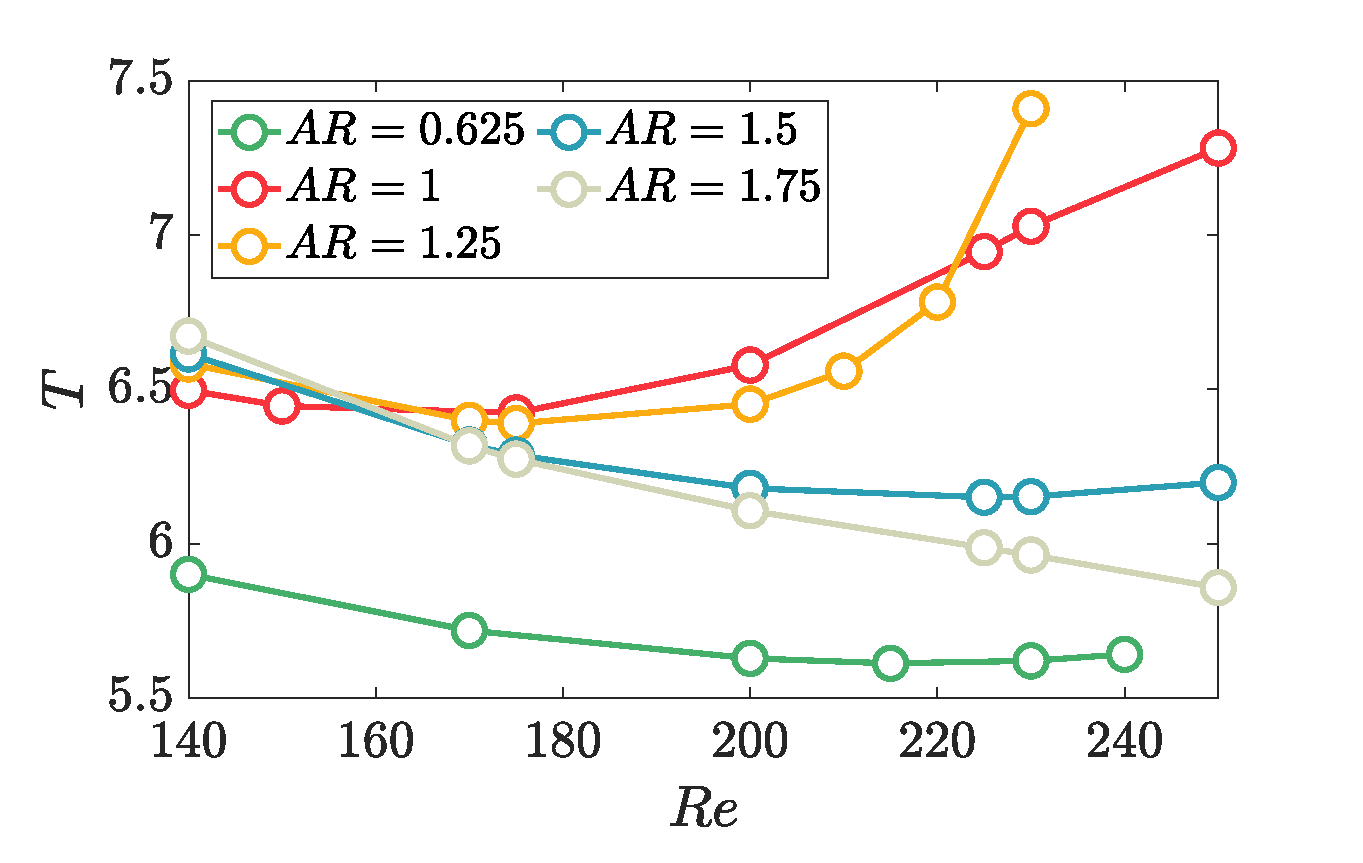
\includegraphics[width=0.49\textwidth]{./fig/AR1s/T_Re.eps}
  \caption{Period of the limit cycle for $1 \le \AR \le 1.75$ as a function of the Reynolds number. XX ADD (i) PANEL WITH DEPENDENCE OF $T$ ON $\AR$ FOR A SELECTED $Re$. (ii) PANEL WITH DEPENDENCE OF THE AERODYNAMIC FORCES on $\AR$ and $Re$. (iii) PANEL WITH DEPENDENCE OF MEAN-FLOW QUANTITIES ON $\AR$ and $Re$. XX}
  \label{fig:T_Re_small}
\end{figure}
%
For $Re>Re_{c2}$ the stability scenario becomes more complex, as the influence of $Re$ on the base-flow topology varies with $\AR$. This trend is clearly illustrated in figure \ref{fig:T_Re_small}, which shows the dependence of the base-flow shedding period $T$ on both $Re$ and $\AR$. For the shortest and logest bodies, $T$ exhibits only minor variations with increase $Re$: it increases by approximately $xx\%$ for $\AR =1$ and decreases by about $xx\%$ for $\AR=1.75$. In contrast, intermediated aspect ratios ($\AR=1.25$) show a mouch stornger dependence on $Re$. Here, $T$ increases significantly with $Re$ rising from $T \approx 6.5$ at $Re \le 210$ to $T \approx 9$ at $Re \ge 250$. This shift reflects changes in the base-flow topology and coincides with the emergence of new instability modes. %The differing sensitivity of the base-flow to $Re$ is further quantified in figure~\ref{fig:T_Re_small}(c-d) which shows the aerodynamics forces and characterstic mean-flow length scales.

\begin{figure}
  \centering
  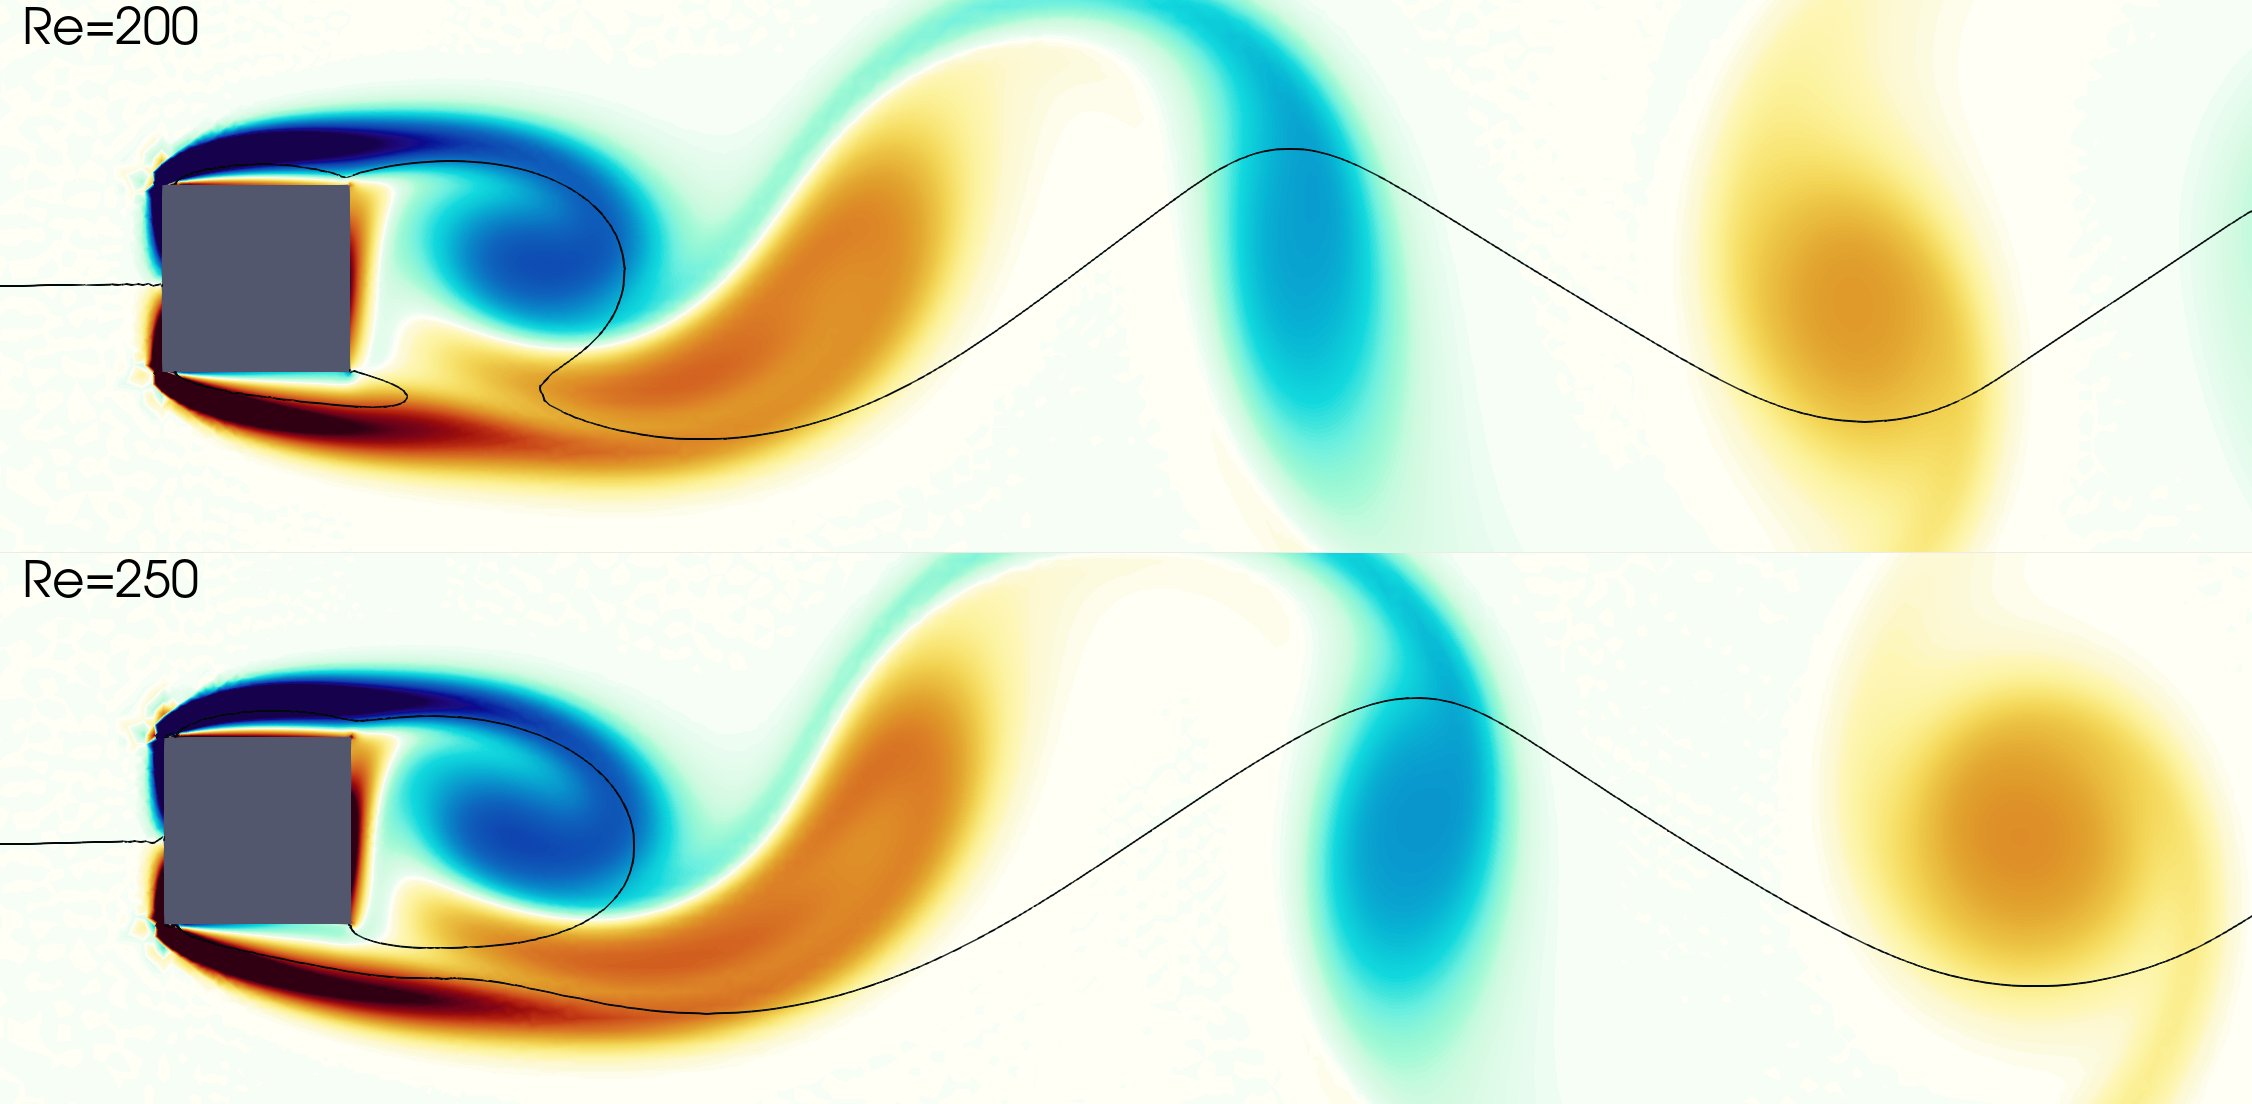
\includegraphics[width=0.49\textwidth]{./fig/AR1/snap/snap.0030.png}
  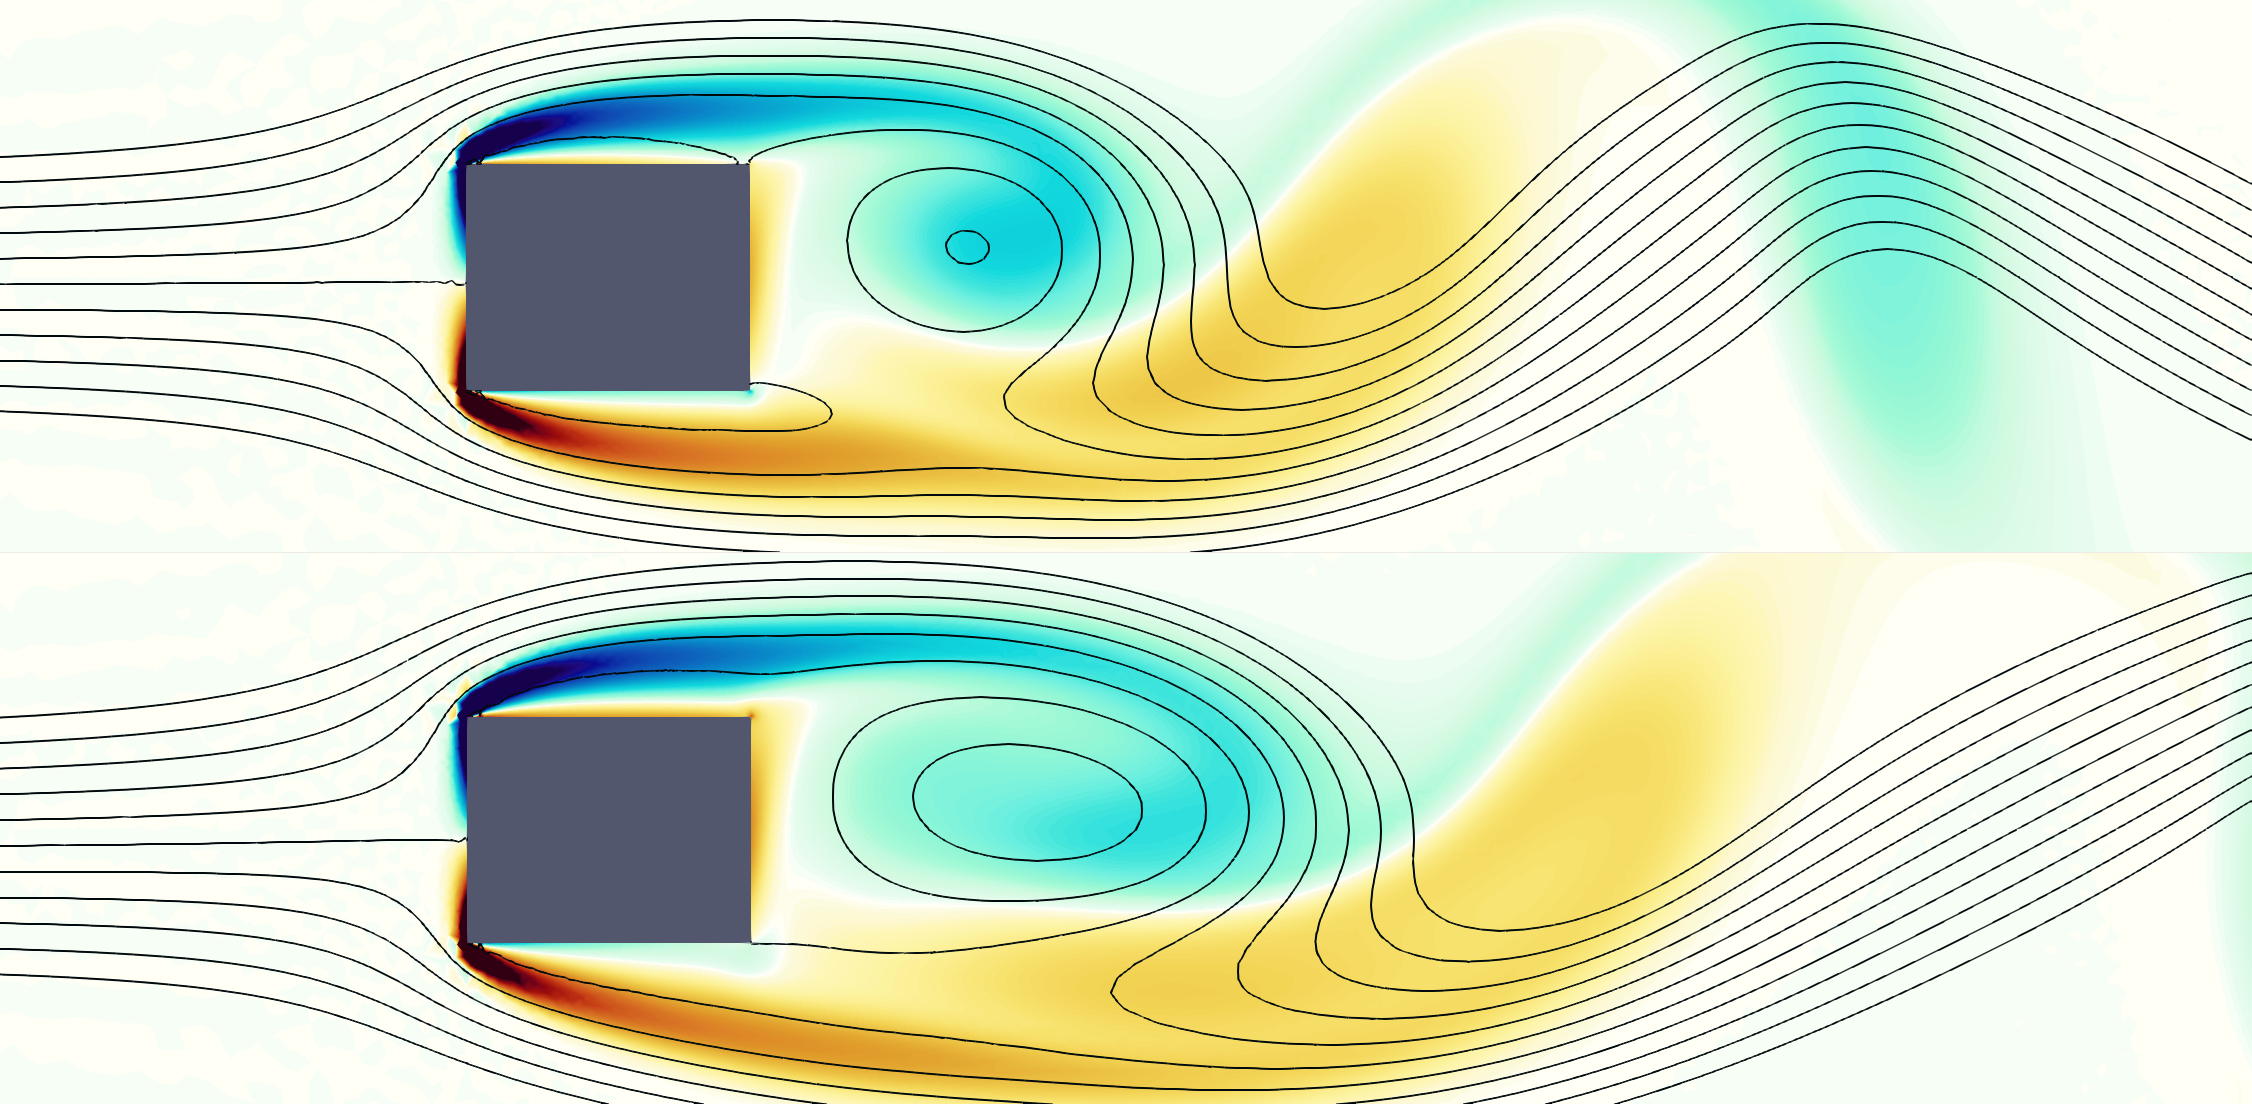
\includegraphics[width=0.49\textwidth]{./fig/AR1p25/snap/snap.0030.png}
  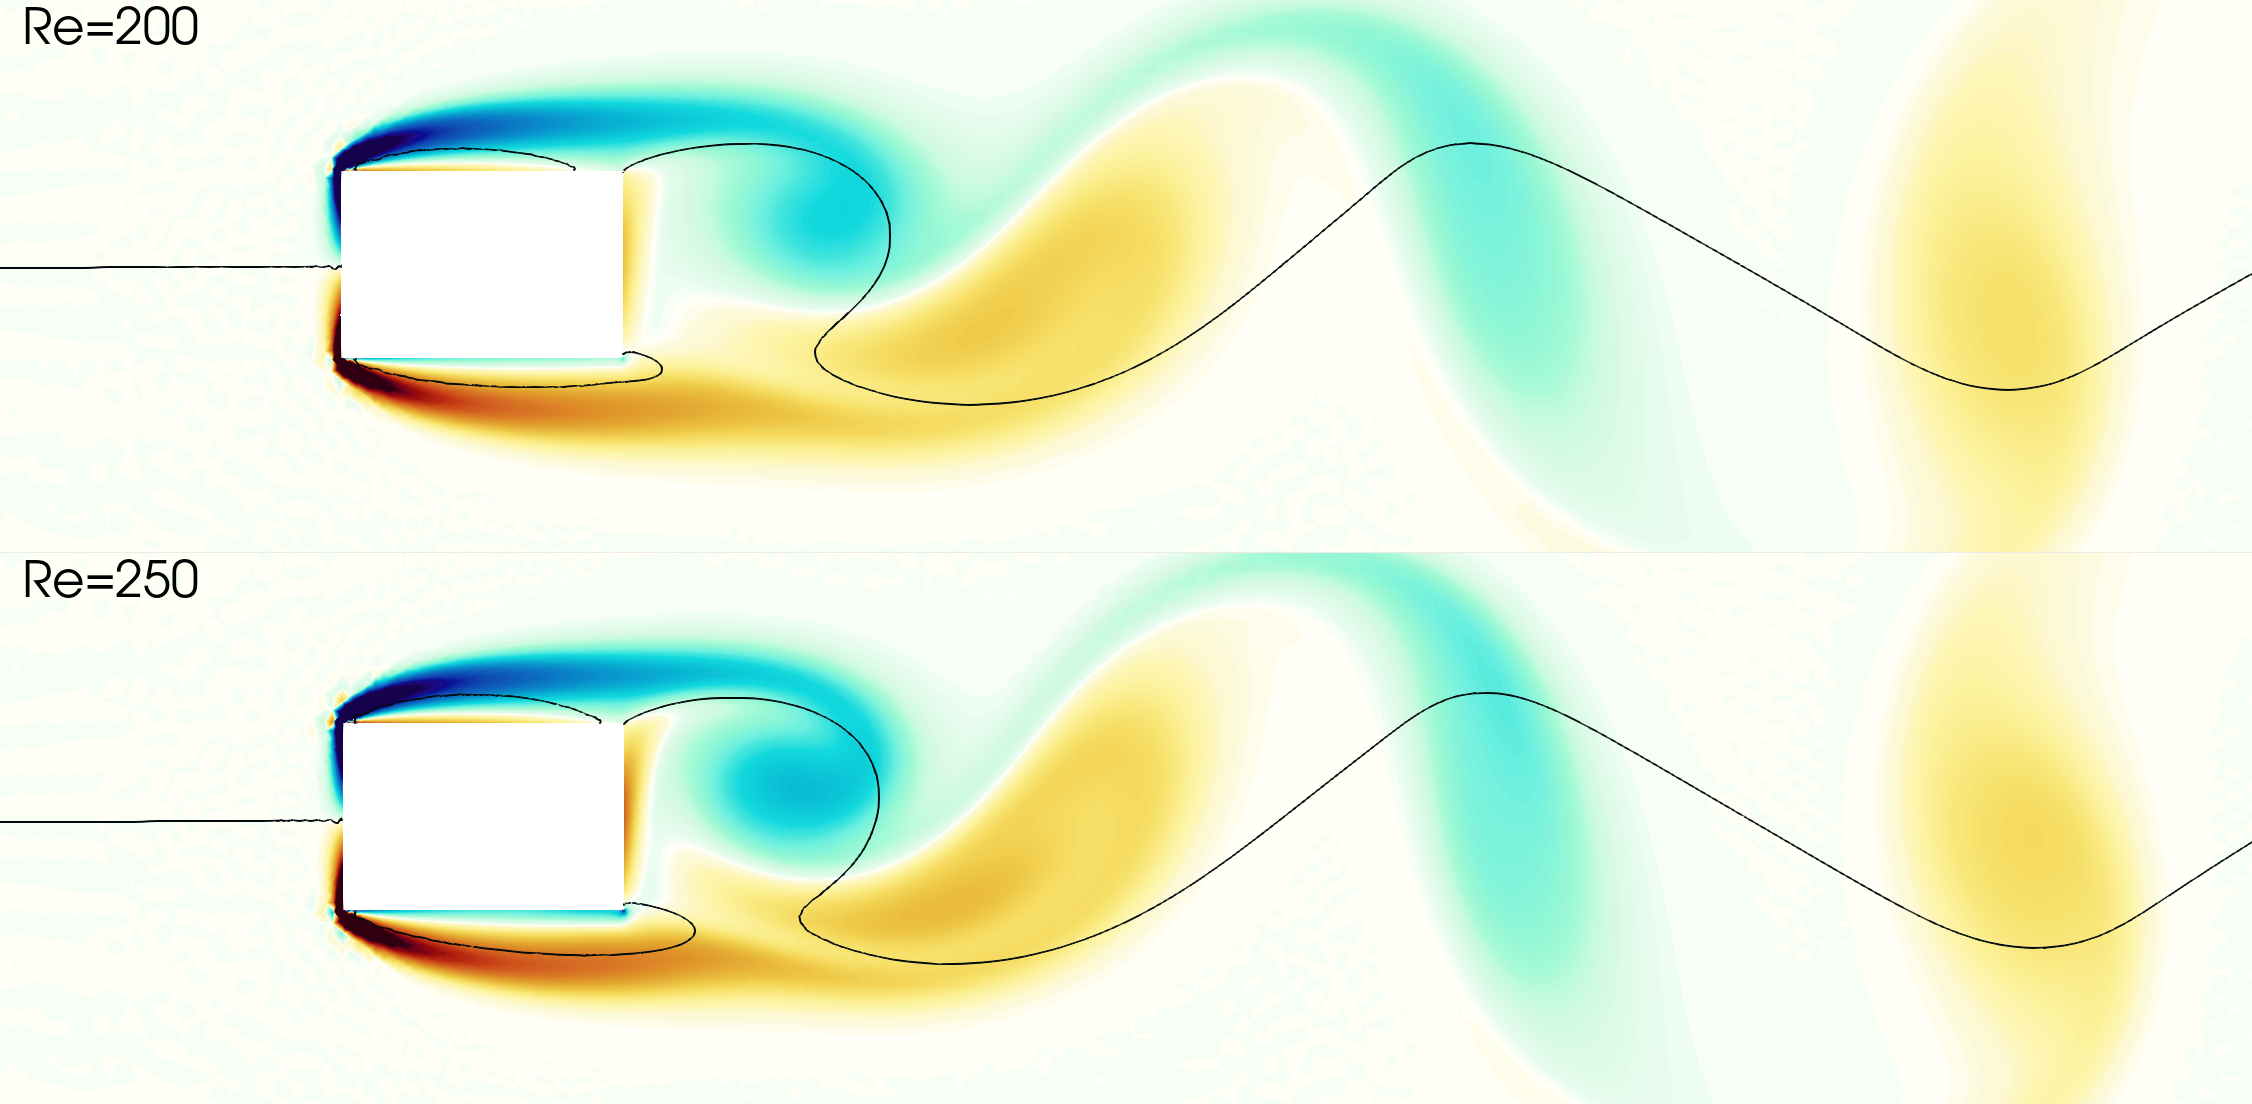
\includegraphics[width=0.49\textwidth]{./fig/AR1p5/snap/snap.0030.png}
  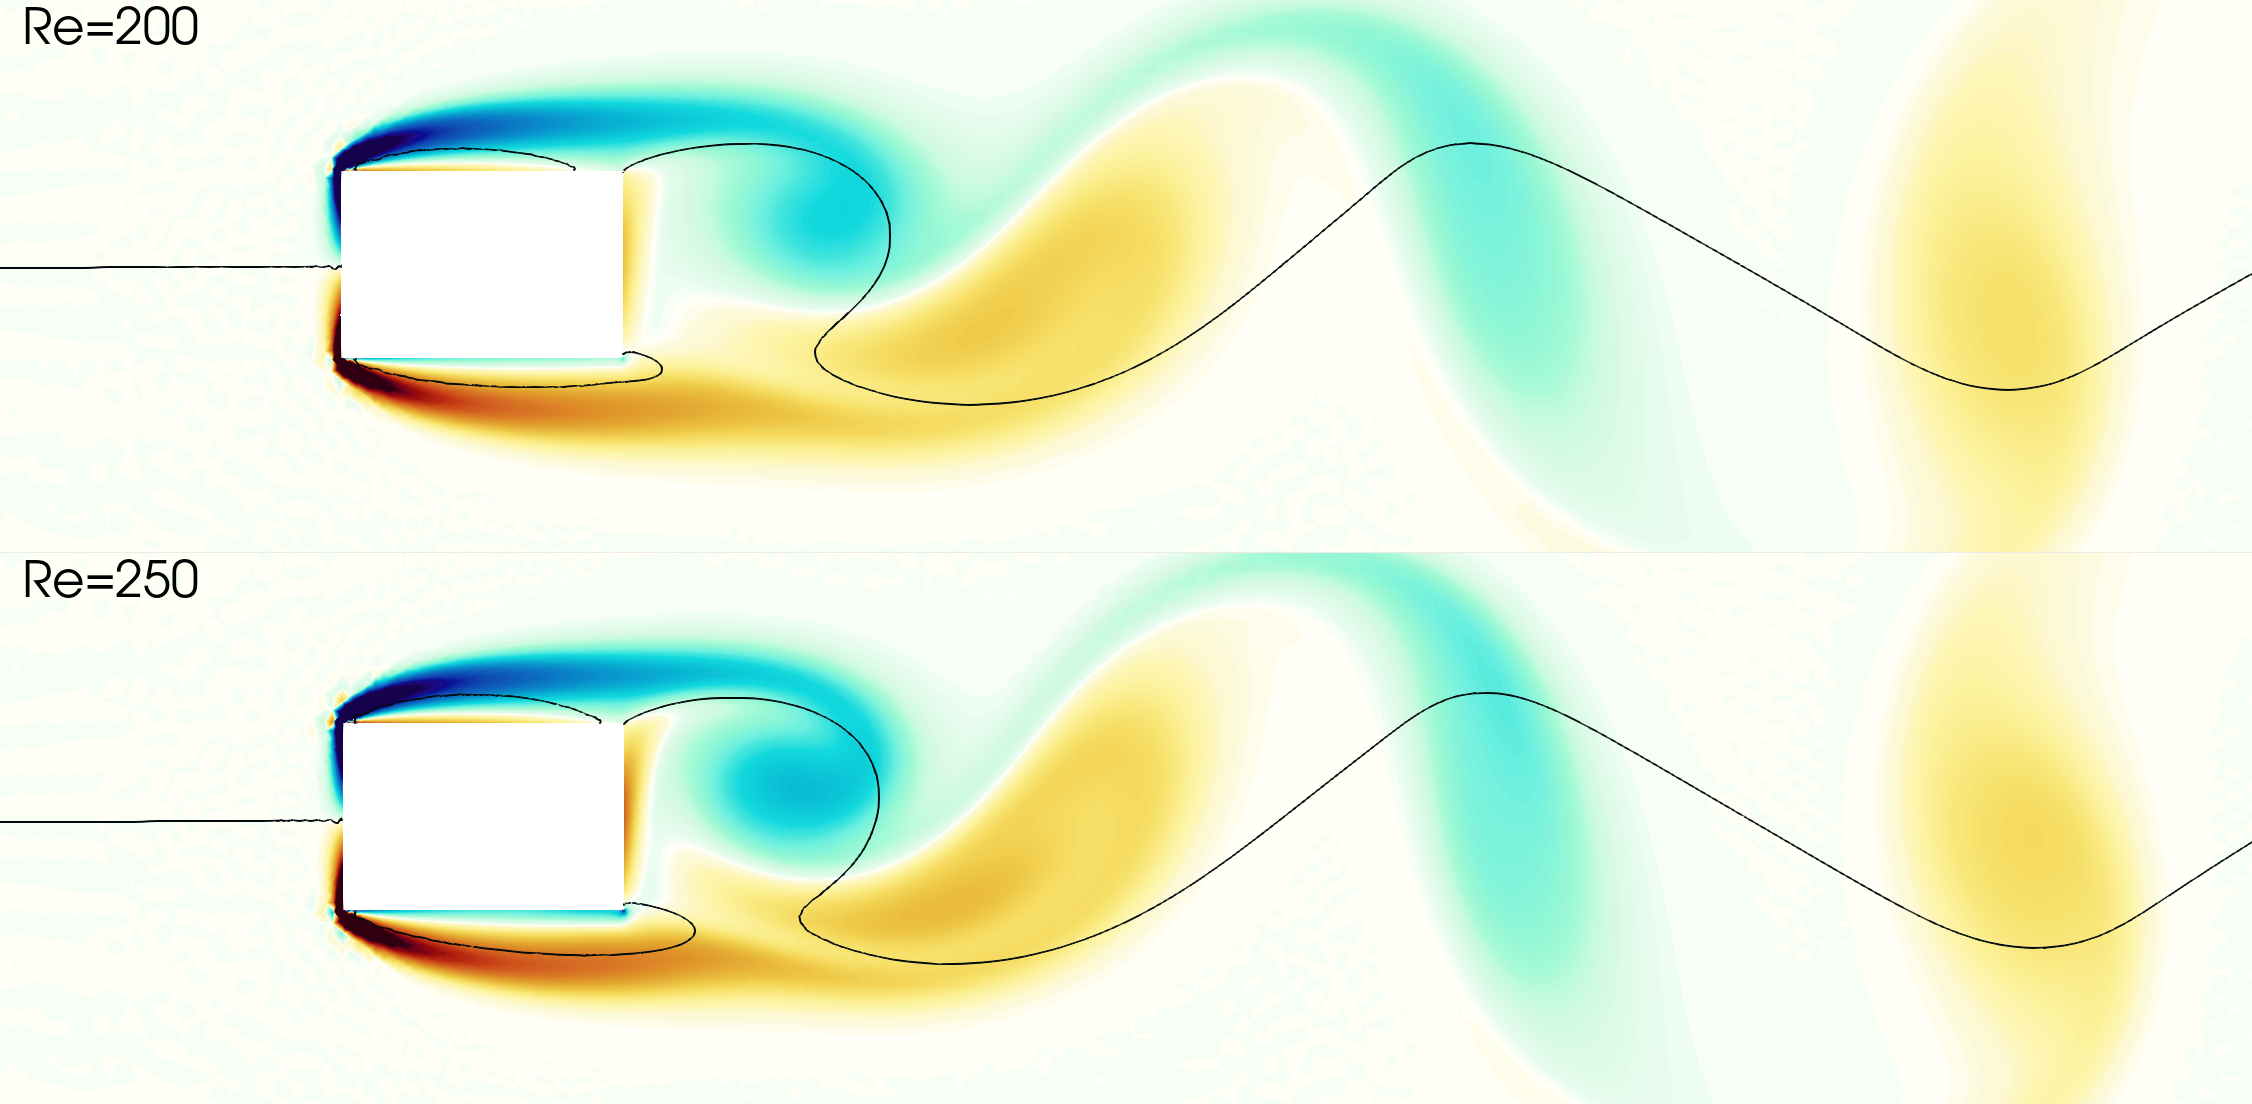
\includegraphics[width=0.49\textwidth]{./fig/AR1p5/snap/snap.0030.png}  
  \caption{Instantaneous snapshots of the base-flow vorticity for $\AR=1$ (top left), $\AR=1.25$ (top right), $\AR=1.5$ (bottom left) and $\AR=1.75$ (bottom right) at $Re=200$ (top) and $Re=250$ (bottom). For all cases the snapshots are taken at the same phase, i.e. just before the shedding of a vortex with negative vorticity in the wake. XX REPLACE $\AR=1.75$ AND ORGANISE THE FIGURE FROM TOP TO BOTTOMXX}
  \label{fig:bf-short}
\end{figure}
%
The influence of $\AR$ on the base-flow topology is shown in figure \ref{fig:bf-short}. For the smaller $\AR < 1.25$, for all considered $Re$ the flow separates at the LE and only intermittently reattaches along the lateral sides of the body. In this case the vortex shedding in the wake is thus determined by the dynamics of the LE shear which is indeed active in the formation of the wake vortex. This is visualised in the figure \ref{fig:bf-short} by the streamline separating from the LE that indeed delimits the wake vortex before it is shed in the wake. For the larger $\AR>1.25$, instead, the LE shear layer reattaches along the lateral sides of the body at all $Re$, and the wake dynamics is determined by the TE shear layer.
By contrast, for the intermediate $\AR=1.25$ the base-flow topology changes with $Re$. At the lower $Re \le 210$ the flow resembles what has been observed for longer bodies, and the wake vortex shedding is driven by the TE shear layers. At the higher $Re>210$, instead, the flow recovers the low-$\AR$ topology, with the wake dynamics being driven by the LE shear layers. This is visualised in figure \ref{}, when comparing panels xx and xx and noting that the streamline separating at the LE corner reattaches for $Re=200$, but not for $Re=250$. This change of topology is explains with the fact that an increase of $Re$ leads to an increase of the angle with which the flow separates at the LE corners, moving thus progressively the reattaching point downtream towards the TE.

To further highlight the change of the flow topology with $\AR$ and $Re$, we look at the mean flow averaged over one shedding period. XX ADD COMMENT SU CAMPO MEDIO + ANDAMENTO DELLE QUANTITA PRINCIPALI XX


 This different base-flow topology influences the size of the wake recirculating region (see figure \ref{}) and explains the different dependence of $T$ on $Re$ for shorter and longer bodies. For shorter bodies $\AR \le 1.25$ an increase of $\AR$ and $Re$ leads to an increase of the angle with which the flow separates at the LE corner resulting thus into a longer mean wake recirculating region $\ell_w$ (which is where the global intability that gives origin to the vortex shedding takes place; see the following), and thus to a lower flow frequency $f \sim \mathcal{U}/\ell_w$ with $\mathcal{U}$ denoting a given time scale. For longer bodies $\AR \ge 1.25$, instead, an increase of $Re$ or $\AR$ results into a shorter wake recirculating region, and thus to a higher flow frequency. Owing to viscous diffusion, indeed, the two shear LE shear layers become thicker in the region downstream the TE as $\AR$ increases as its distance from the LE increases, inducing a quicker close of the mean-flow streamlines. 
  
XX FIGURE CON EIGENMODE E SENSITIVITA. FAI VEDERE $Re=200$ e $Re=250$ per $\AR=1$ e $\AR=1.5$ e $Re=200$ e $Re=230$ per $\AR=1.25$. \textcolor{red}{DOBBIAMO FARE $Re=230$ per $\AR=1$ e $\AR=1.5$?} XX

To further highlight the change of the flow topology with $\AR$ and $Re$, we perform a global stability analysis of the mean flow averaged over one shedding period. The focus in on the leading eigenmode, which is representative of the unsteady phenomena of the flow. For a similar approach see for example \cite{pier-2002,barkley-2006} for the circular cylinder and \cite{chiarini-quadrio-auteri-2022} for rectangular cylinders. 
%
The frequency of the leading eigenmode predicts fairly well the Strouhal number observed in the nonlinear simulations for all cases, with a maximum difference of $xx\%$. Unlike the case of the circular cylinder, which is marignally stably \citep{barkley-2006}, the present mean flow stability analysis leads to a slightly negative $\sigma$. Figure \ref{}, shows the real part of the cross-stream velocity component of the leading eigenmode (left) and its structural sensitivity (right) introduced by \cite{giannetti-luchini-2007}. For large $\AR$ and for intermediate $\AR=1.25$ at small $Re$ the eigenmode is visible only after the TE. By contrast, for smaller $\AR$ and for larger $Re$ the eigenmode is non negligible also over the lateral sides of the cylinder, indicatng that in these cases the LE shear layers play a role in the vortex shedding dynamics. This observation is further confirmed by the structural sensitivity. The structural sensitivity identifies the flow region where structural modifications of the stability problem produce the strongest drift of the leading eigenvalue and indentifies the so-called wavemaker. The largest values of the sensitivity occur near the cylinders, as the
product of the adjoint and direct modes is small in the remaining part of the domain. For longer bodies and smaller $Re$ non null values are observed only in the wake behind the TE along the streamline delimiting the mean recirculating region. The core of the instability responsible for the TE vortex shedding is located downstream the TE. For shorter bodies and/or larger $Re$ the structural sensitivity is non negligible also along the LE shear layers over the lateral sides of the cylinder. Accordingly, in these cases the wavemaker extends to the LE shear layers.

\begin{figure}
  \centering
  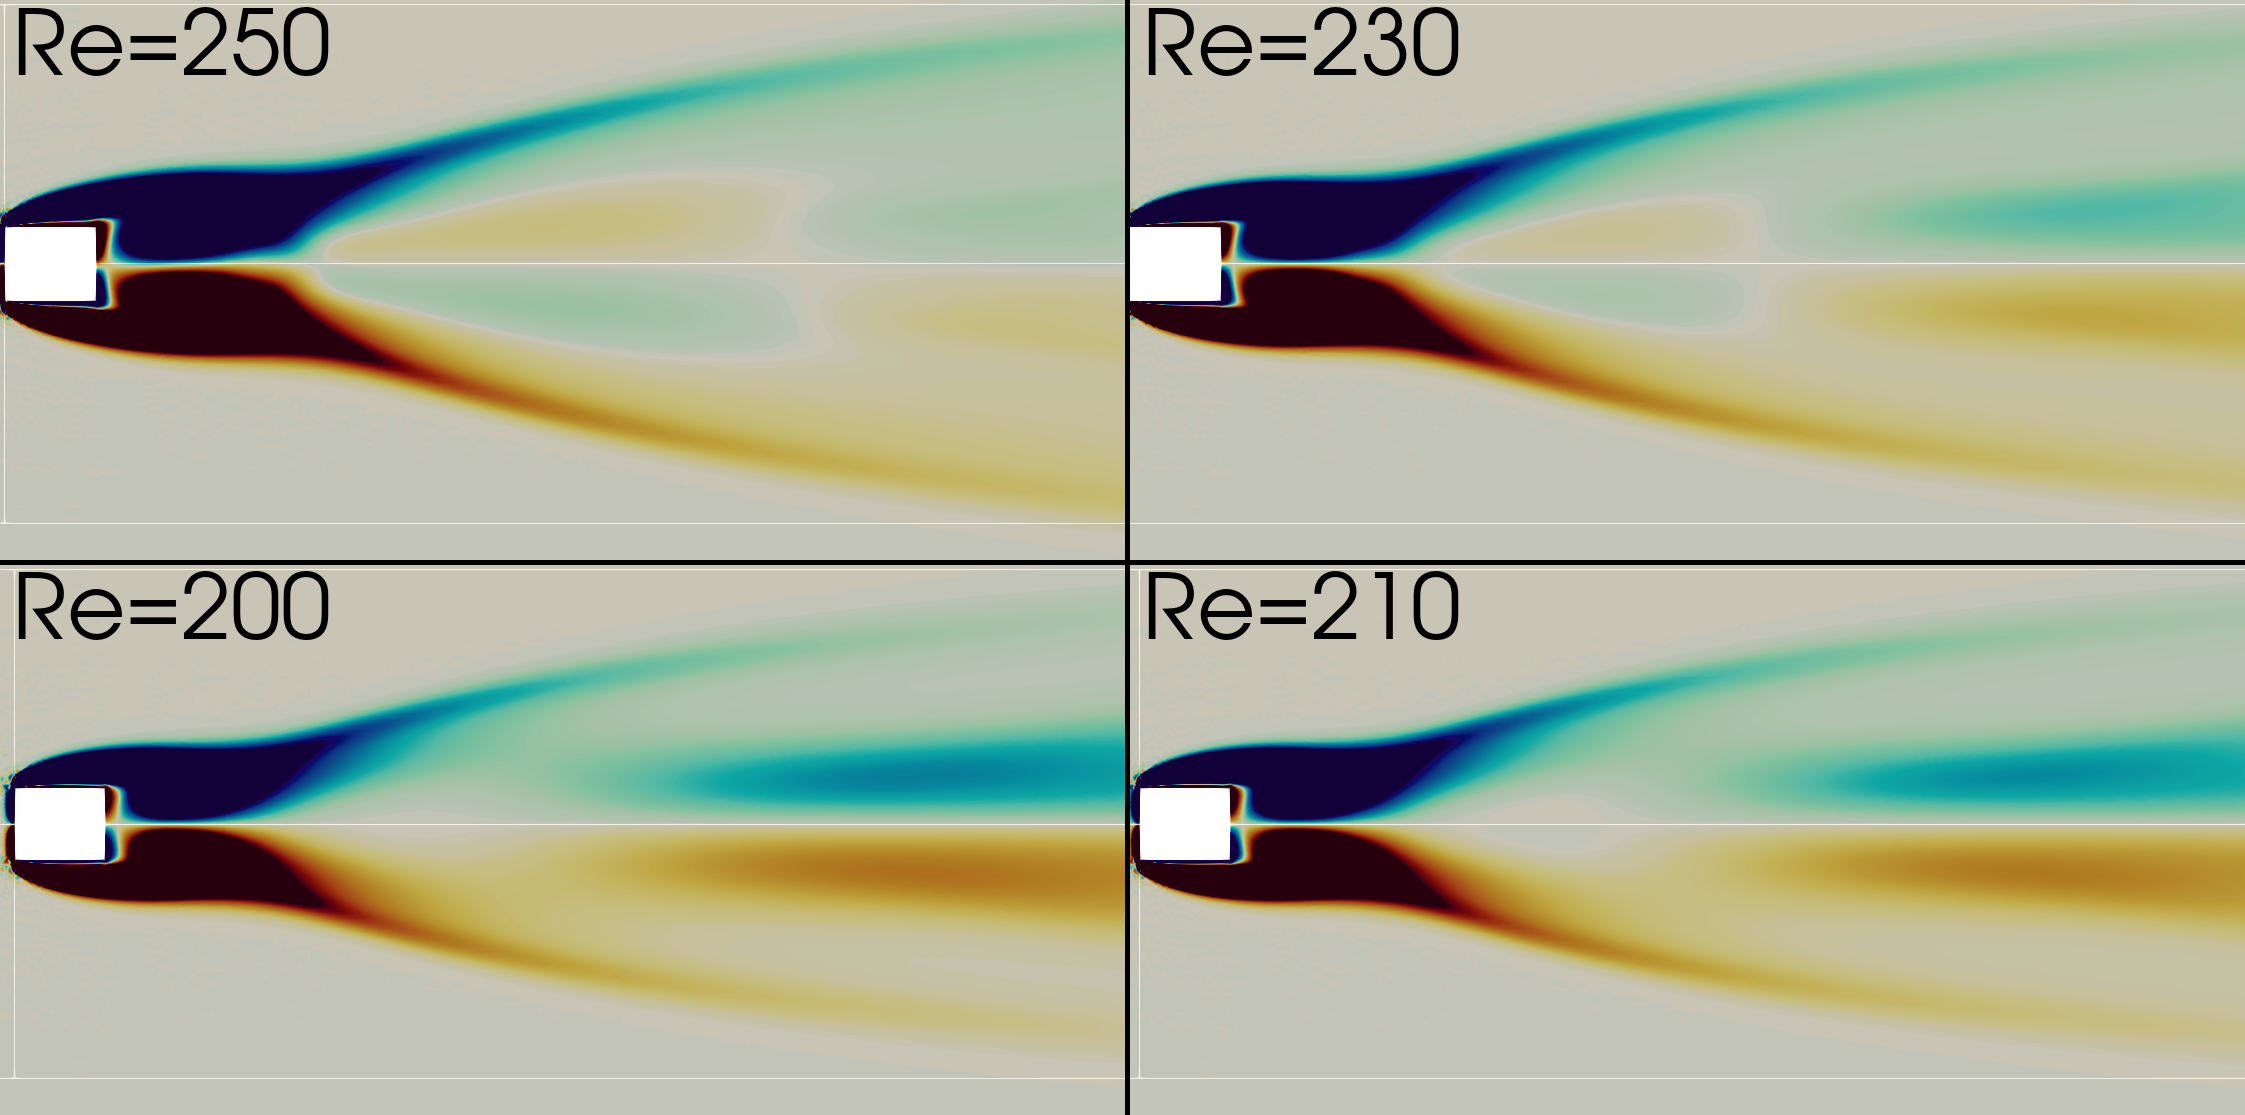
\includegraphics[width=0.9\textwidth]{./fig/AR1p25/Av_BF_Re200_Re250.png}
  \caption{Average base-flow vorticity for $\AR=1.25$ and $200 \le Re \le 250$.}
  \label{fig:av_bf}
\end{figure}

\begin{figure}
  \centering
  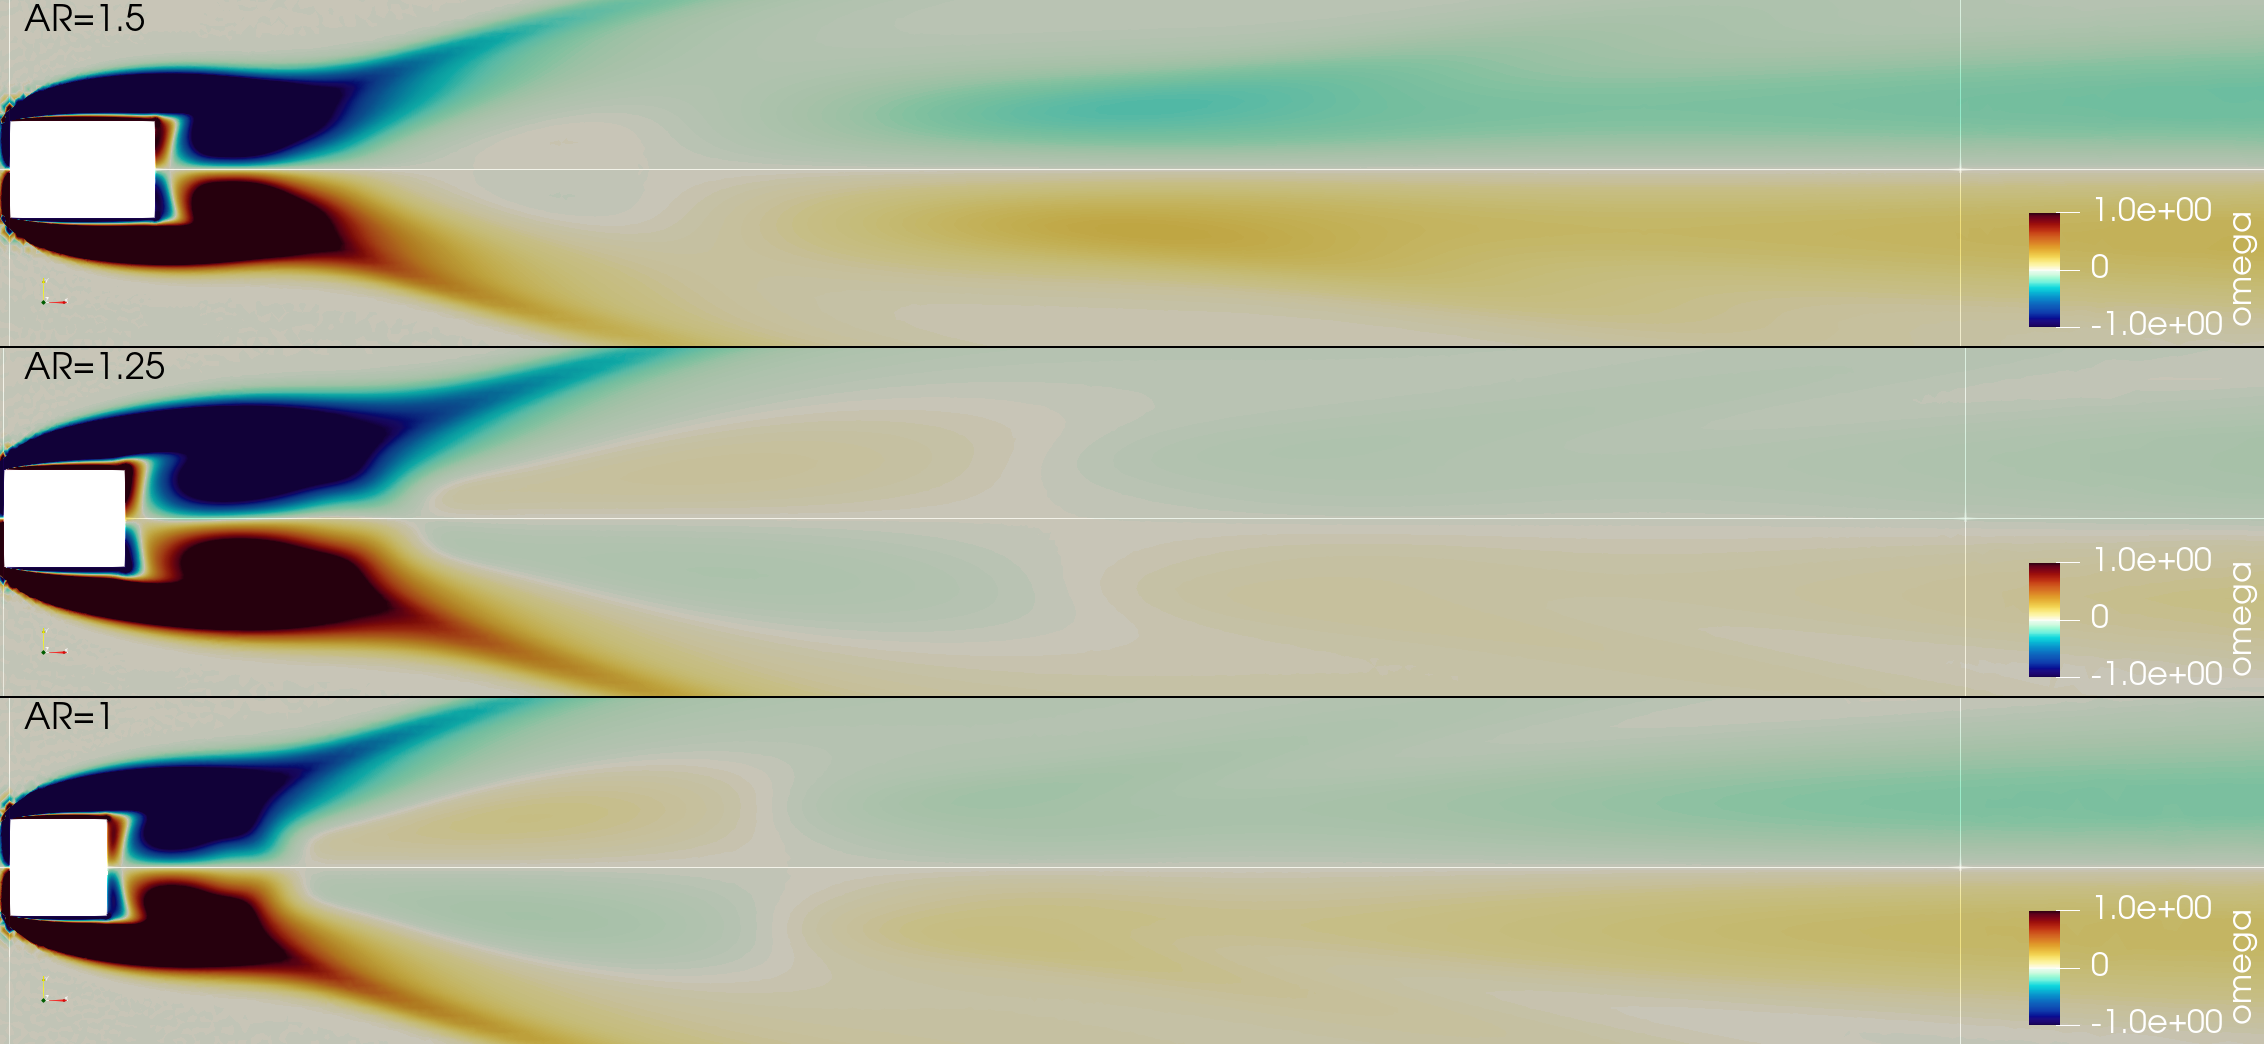
\includegraphics[width=0.9\textwidth]{./fig/AR1s/mean_vort_Re250.png}
  \caption{Average base-flow vorticity for $Re=25$ and $1 \le \AR \le 1.5$.}
  \label{fig:av_bf2}
\end{figure}

\begin{figure}
  \centering
  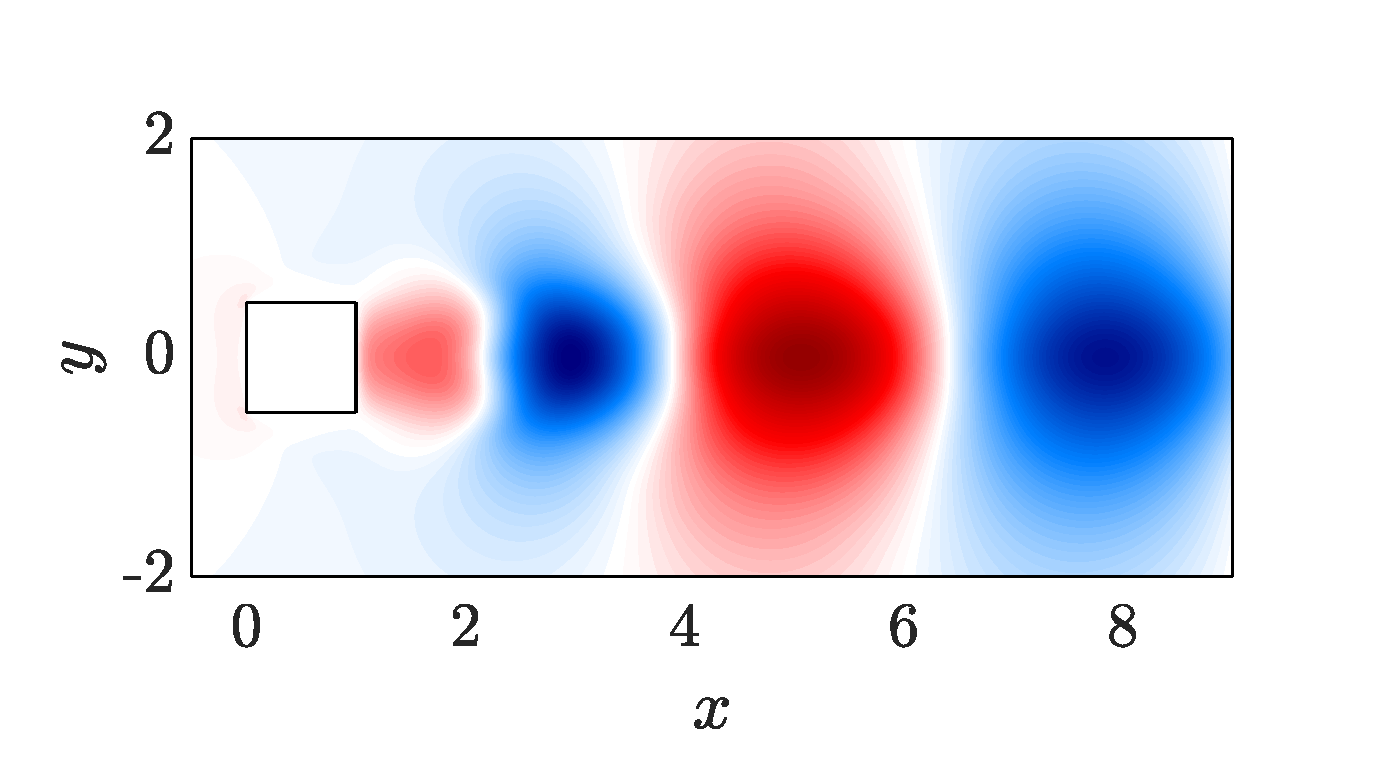
\includegraphics[width=0.49\textwidth]{./fig/AR1/LinStab/v_Re200.eps}
  \includegraphics[width=0.49\textwidth]{./fig/AR1/LinStab/sens_Re200.eps}
  \includegraphics[width=0.49\textwidth]{./fig/AR1p25/LinStab/v_Re200.eps}
  \includegraphics[width=0.49\textwidth]{./fig/AR1p25/LinStab/sens_Re200.eps}
  \includegraphics[width=0.49\textwidth]{./fig/AR1p5/LinStab/v_Re200.eps}
  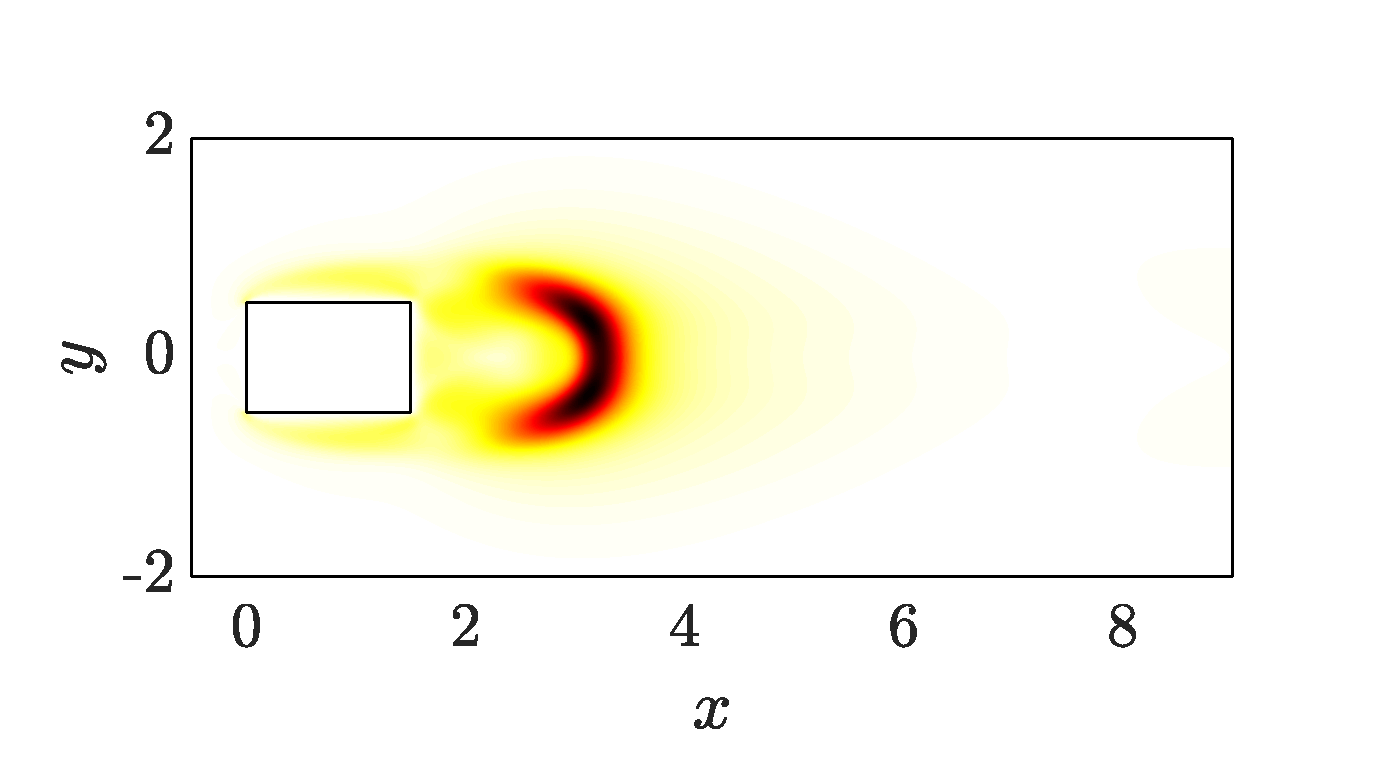
\includegraphics[width=0.49\textwidth]{./fig/AR1p5/LinStab/sens_Re200.eps}
  \caption{Linear stability analysis of the mean flow for $Re=200$. Left: vertical velocity. Right: Structural sensitivity. Top: $\AR=1$. Centre: $\AR=1.25$. Bottom: $\AR=1.5$.}
  \label{fig:MF_stab3}
\end{figure}

\begin{figure}
  \centering
  \includegraphics[width=0.49\textwidth]{./fig/AR1/LinStab/v_Re250.eps}
  \includegraphics[width=0.49\textwidth]{./fig/AR1/LinStab/sens_Re250.eps}
  \includegraphics[width=0.49\textwidth]{./fig/AR1p25/LinStab/v_Re250.eps}
  \includegraphics[width=0.49\textwidth]{./fig/AR1p25/LinStab/sens_Re250.eps}
  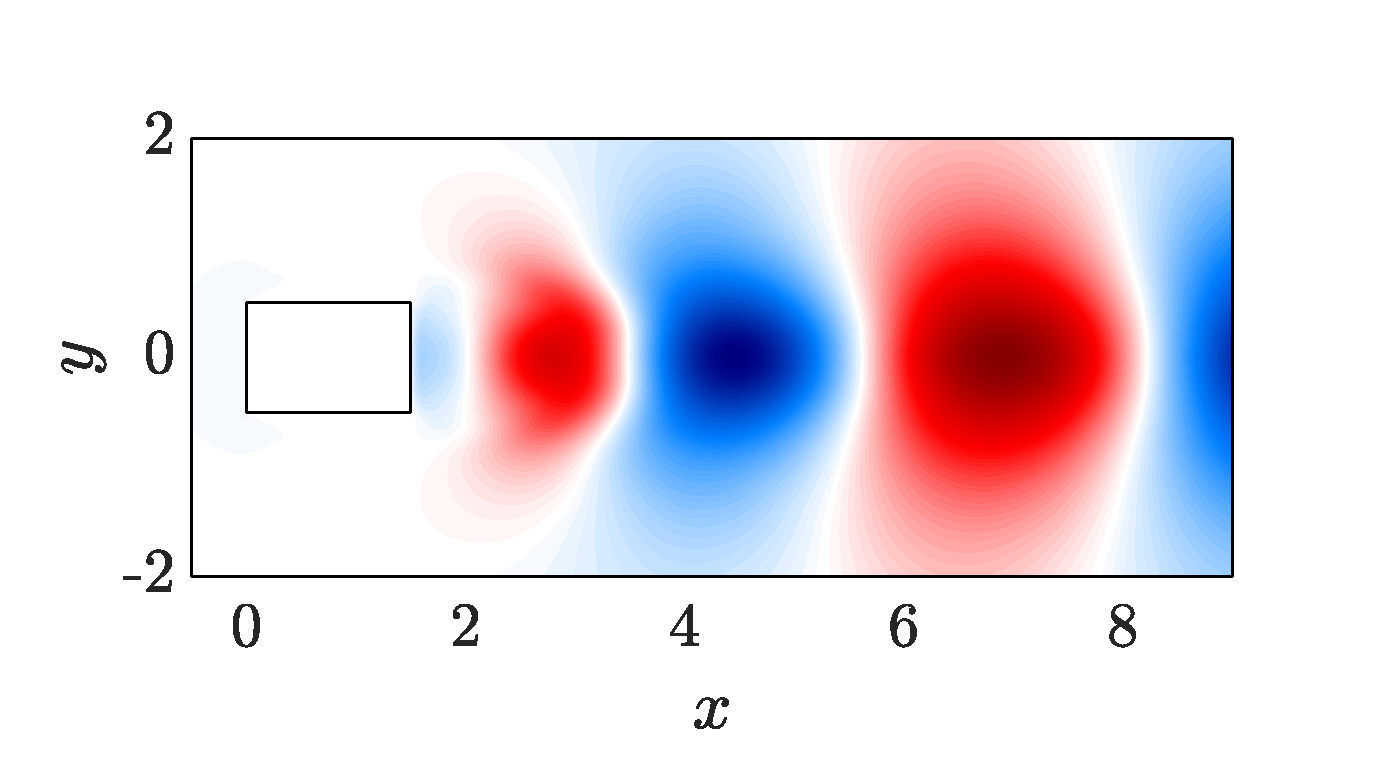
\includegraphics[width=0.49\textwidth]{./fig/AR1p5/LinStab/v_Re250.eps}
  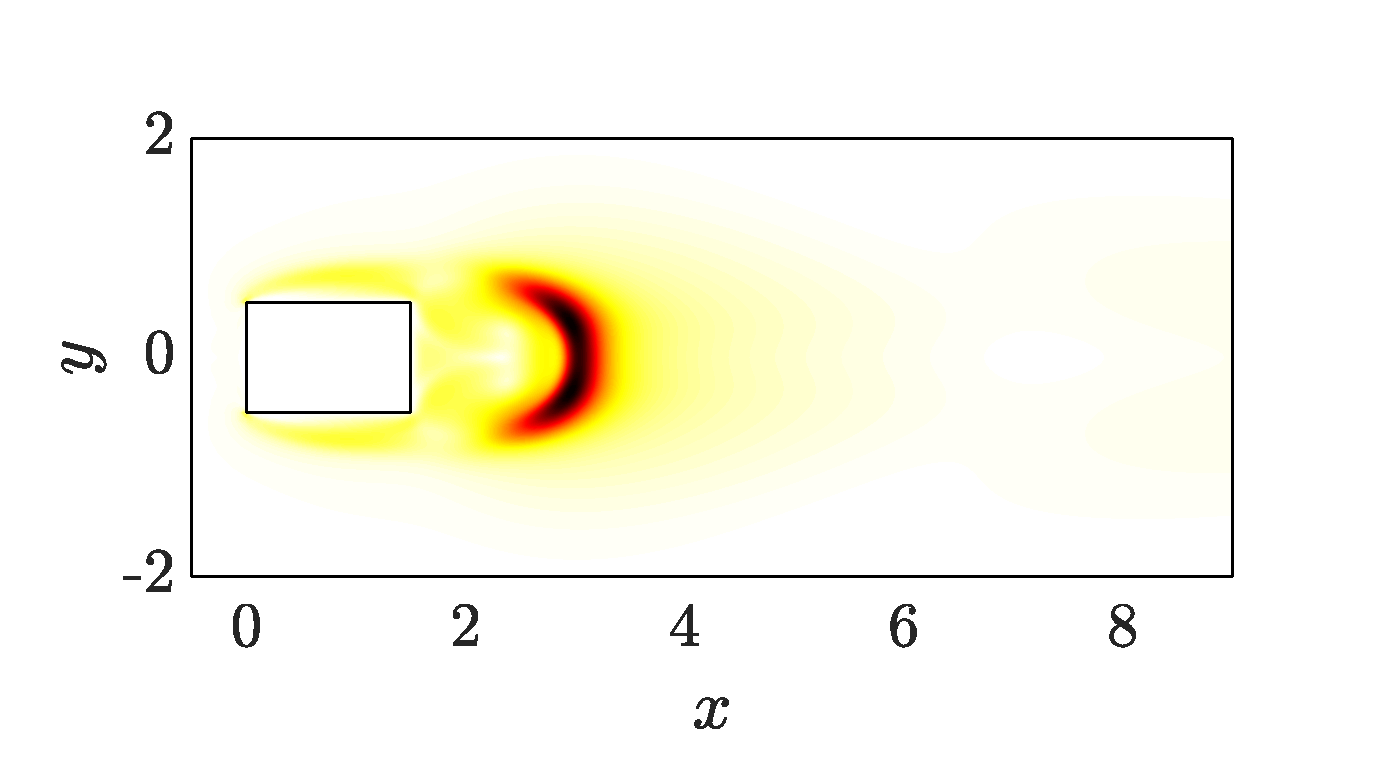
\includegraphics[width=0.49\textwidth]{./fig/AR1p5/LinStab/sens_Re250.eps}
  \caption{Linear stability analysis of the mean flow for $Re=250$. Left: vertical velocity. Right: Structural sensitivity. Top: $\AR=1$. Centre: $\AR=1.25$. Bottom: $\AR=1.5$. XX SEMBREREBBE CHE IL CAMBIO DI TREND SIA DOVUTO AL FATTO CHE LO LE SHEAR LAYER PARTECIPI AL VS PER AR PICCOLI E NON PER AR GRANDI. ALL'AUMENTARE DI RE ANGOLO DI SEPARAZIONE TENDE AD AUMENTARE, COSI COME LA DIM DELLA BOLLA SOPRA AL CORPO. PER AR GRANDI PERO L'AUMENTO DELLA LUNGHEZZA INIBISCE L'INTERAZIONE TRA IL VS E IL LE SHEAR LAYER. XX GUARDA ANCHE $Re=200$ XX}
  \label{fig:MF_stab2}
\end{figure}

\begin{figure}
  \centering
  \includegraphics[width=0.49\textwidth]{./fig/AR1p25/LinStab/v_Re200.eps}
  \includegraphics[width=0.49\textwidth]{./fig/AR1p25/LinStab/sens_Re200.eps}
  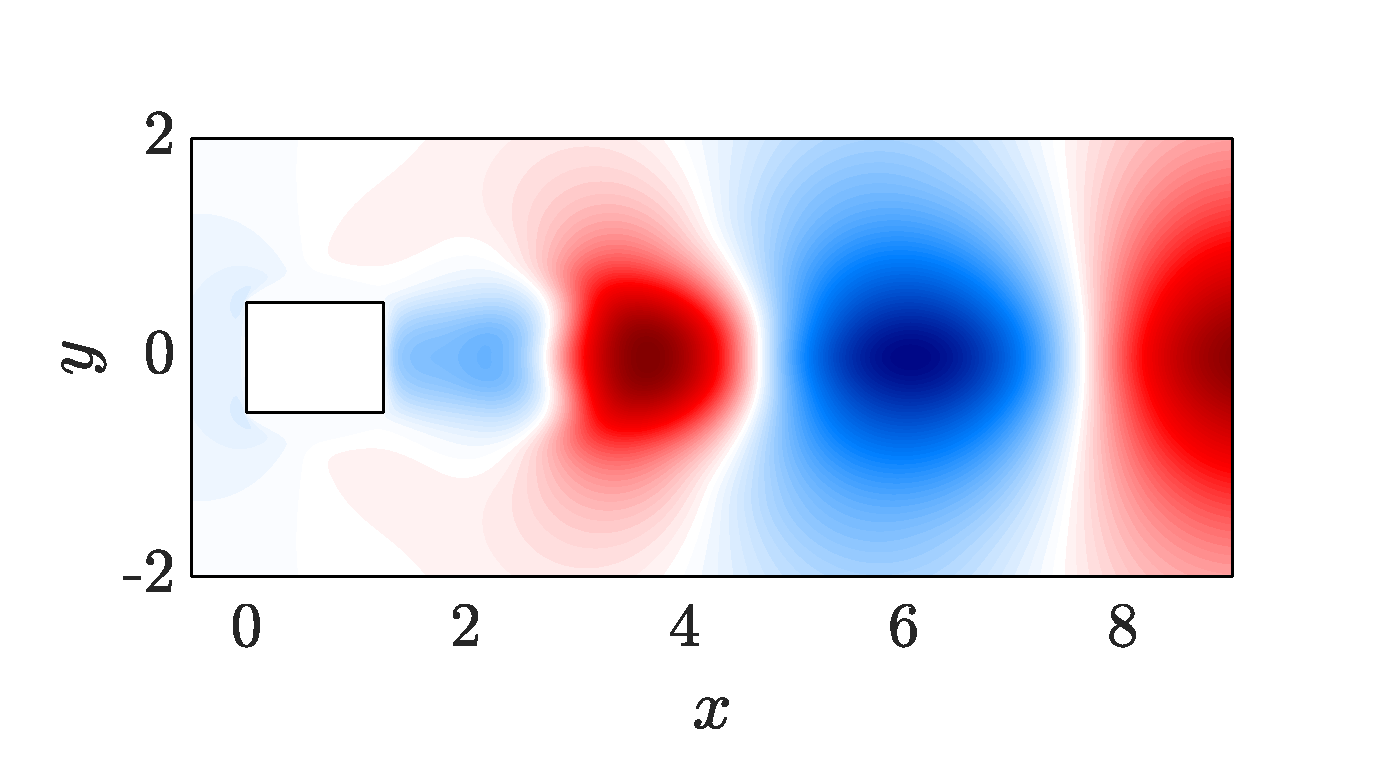
\includegraphics[width=0.49\textwidth]{./fig/AR1p25/LinStab/v_Re230.eps}
  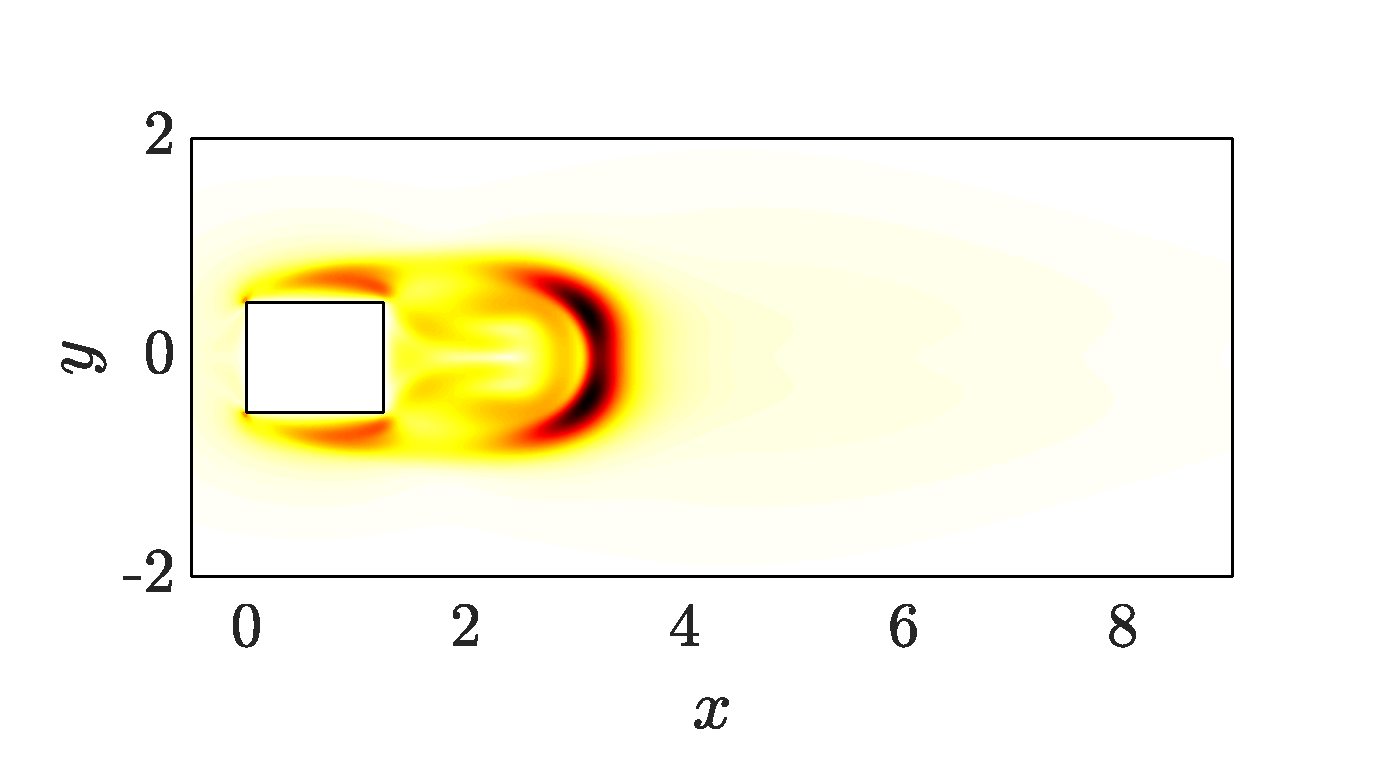
\includegraphics[width=0.49\textwidth]{./fig/AR1p25/LinStab/sens_Re230.eps}
  \includegraphics[width=0.49\textwidth]{./fig/AR1p25/LinStab/v_Re250.eps}
  \includegraphics[width=0.49\textwidth]{./fig/AR1p25/LinStab/sens_Re250.eps}
  \caption{Linear stability analysis of the mean flow for $\AR=1.25$. Left: vertical velocity. Right: Structural sensitivity. Top: $Re=200$. Centre: $Re=230$. Bottom: $Re=250$.}
  \label{fig:MF_stab}
\end{figure}

\subsection{The bifurcations}

\begin{figure}
  \centering
  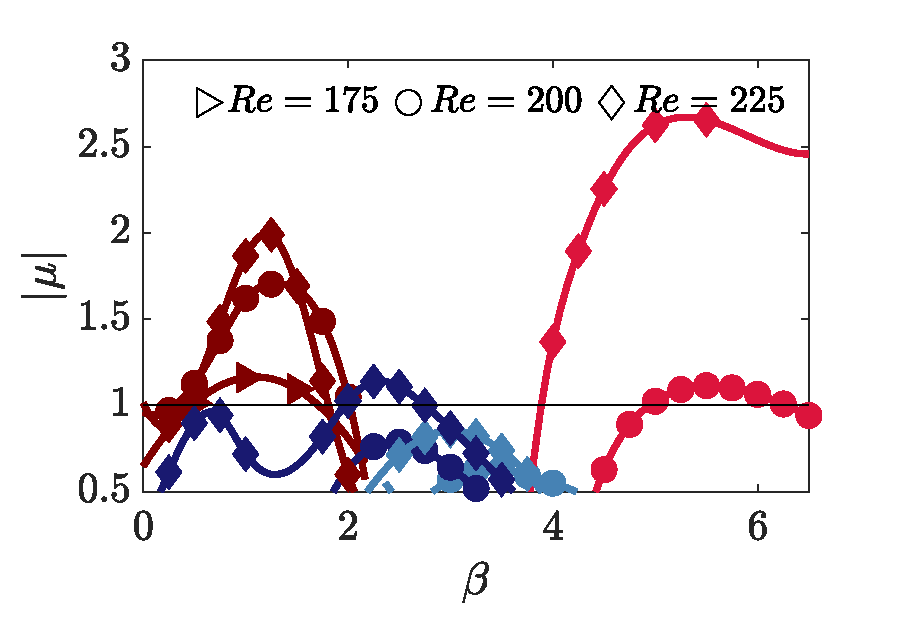
\includegraphics[width=0.49\textwidth]{./fig/AR1/neutralb.eps}
  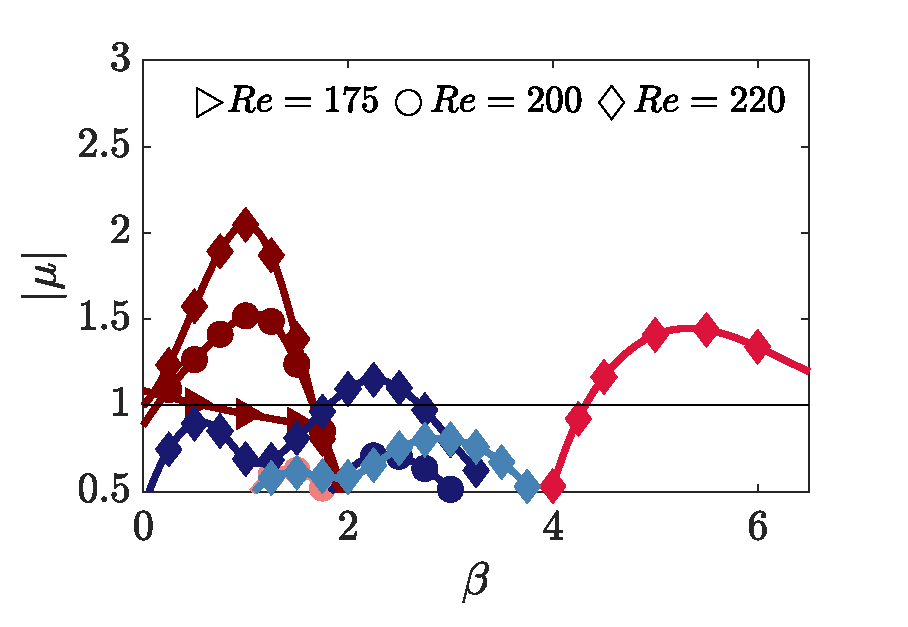
\includegraphics[width=0.49\textwidth]{./fig/AR1p25/neutralb.eps}  
  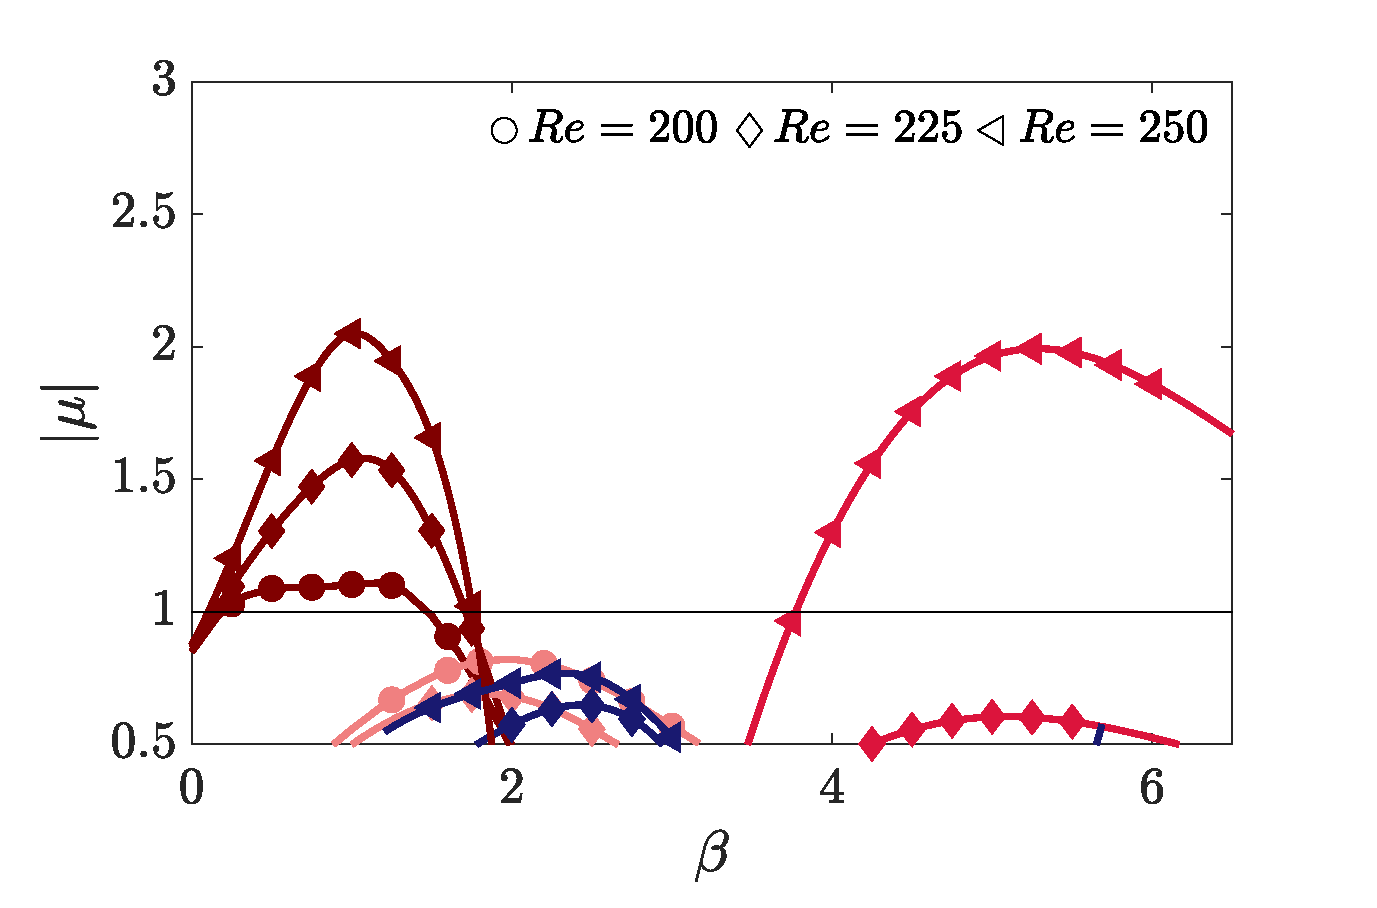
\includegraphics[width=0.49\textwidth]{./fig/AR1p5/neutralb.eps}    
  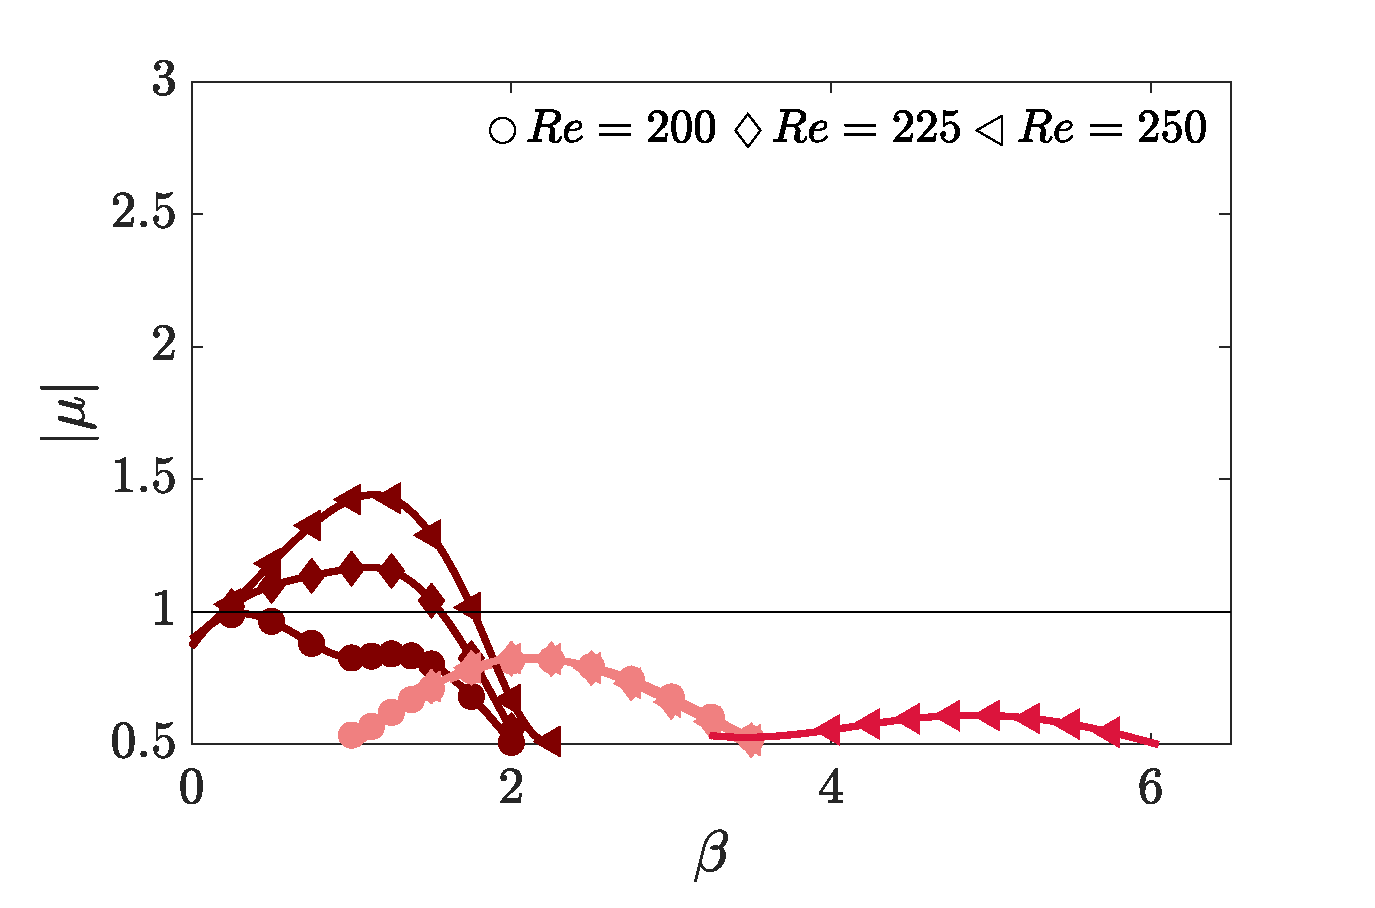
\includegraphics[width=0.49\textwidth]{./fig/AR1p75/neutralb.eps}       
  \caption{Top: multipliers for $\AR=1$, $\AR=1.25$ and $\AR=1.5$ at $Re=200$; the red line refers to mode $A$, the grey line to mode $C$, the green line to mode $B$ and the light blue line refers to mode $B'$. Mode $B'$ has the same spatio-temporal symmetry of mode $B$, but its characteristic wavelength is much smaller, being similar to that of mode $A$. This mode resembles that found for elongated bodies with elliptic leading edge by \cite{ryan-etal-2005}. XX ADD FIGURE CON I MODI XX}
  \label{fig:mult_AR1_AR1p75}
\end{figure}
%
As mentioned in \S\ref{sec:intro}, for $\AR=1$ three distinct modes become unstable in rapid succession. Mode A first becomes unstable at $Re \approx 175$ with a characteristic wavelength of $\lambda_A \approx 5$ ($\beta_A \approx 1.2$) and the following spatio-temporal symmetry 
%
\begin{equation}
  \hat{\omega}_x(x,y,\beta,t) = - \hat{\omega}_x(x,-y,\beta,t+/2)
\end{equation}
%
Mode B becomes unstable at $Re \approx 200$, has a characteristic wavelength $\lambda_B \approx 1$ ($\beta_B \approx 5.8$) and satisfies the symmetry:
%
\begin{equation}
  \hat{\omega}_x(x,y,\beta,t) = + \hat{\omega}_x(x,-y,\beta,t+T/2).
\end{equation}
%
Finally, mode QP becomes unstable at the higher $Re \approx 230$ with a characteristic wavelength of $\lambda_{QP} \approx 2.7$ ($\beta_{QP} \approx 2.3$). These results are in excellent agreement with our findings shown in figure~\ref{fig:mult_AR1_AR1p75}$(a)$, providing a validation of our numerical approach.

Figure~\ref{fig:mult_AR1_AR1p75} illustrates the effect of increasing the aspect ratio. As $\AR$ increases, the onset of secondary instabilities is progressively delayes: fixing $Re$ our results show a consistent decrease inthe modulus of the Floquet multipliers associated with the three known modes, indicating a more stable base flow for longer bodies. Quantitativley, the critical Reynolds number increases from $Re_{c2} \approx 175$ for $\AR=1$ to approximately $Re_{c2} =200-225$ for $\AR=1.75$. This trend aligns with the delyed onset of the primary instability reported by \cite{chiarini-quadrio-auteri-2021}. Despite the stabilising effect, the sequence of bifurcations remains essentially unchanged for $1 \le \AR \le 1.75$, with mode A becoming unstable first, followed by mode B. The characteristic wavelengths of these modes exhibit only martinal variations with $\AR$, consistent with the findings of \cite{choi-yang-2014} for $\AR<1$.

In addition to the three established modes, a new mode, denoted B', emergest for $\AR>1$. Mode B' shares the same spatio-temporal symmetry as mode B, but is characterised by a significantly longer wavelength, comparable to that of mode A; see figure \ref{fig:modes_AR1_AR1p75}. A mode with similar features --- both in wavelength and symmetry --- was previously reported by \cite{ryan-etal-2006} in the wake of elongated bodies with streamlined LE and blunt TE. However, within the parameter range considered here, mode B' remains stable.


\begin{figure}
  \centering
  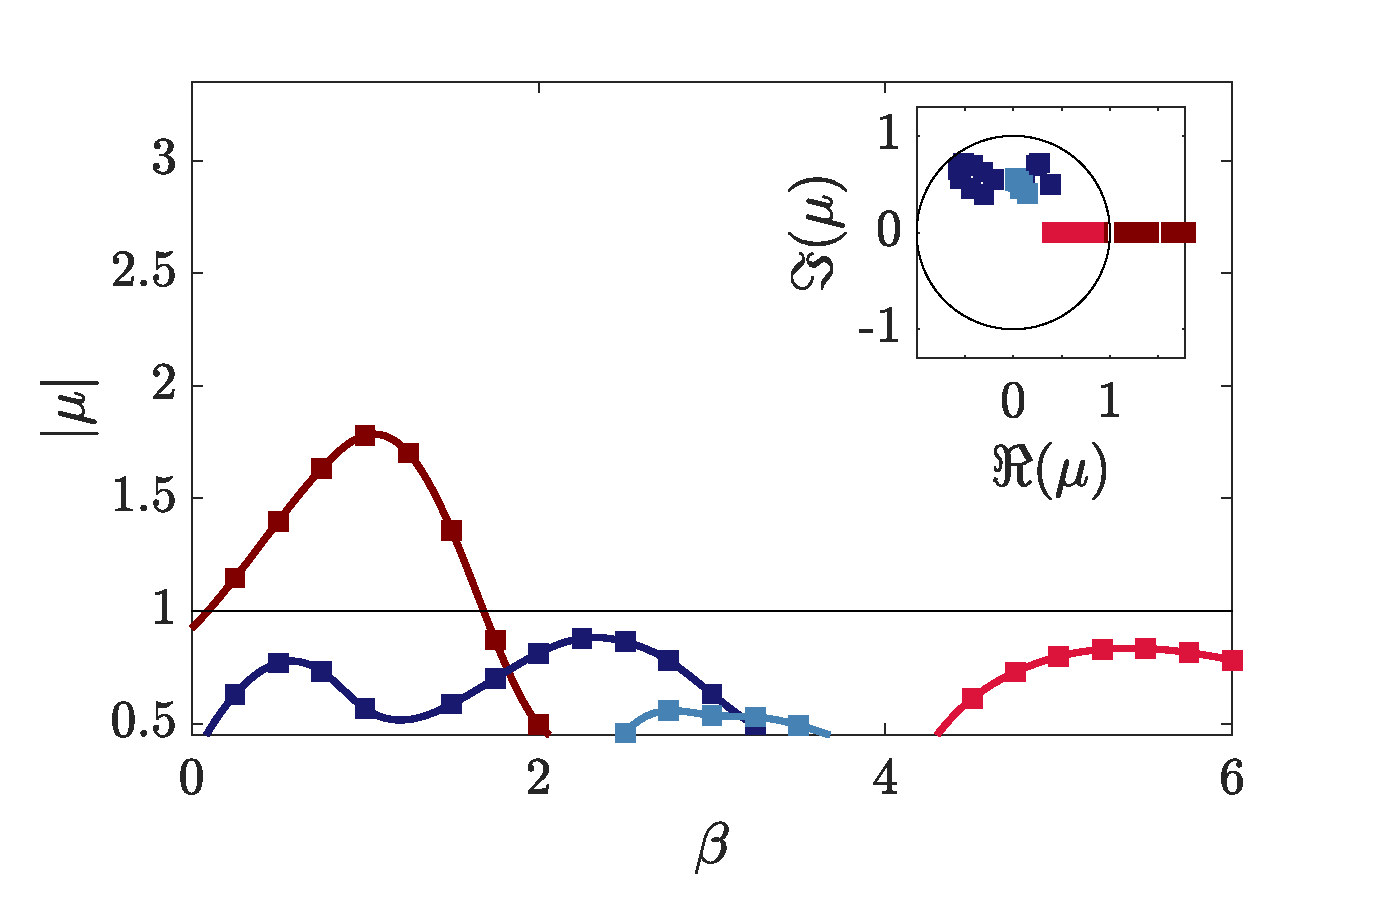
\includegraphics[width=0.49\textwidth]{./fig/AR1p25/mu_beta_Re210.eps}
  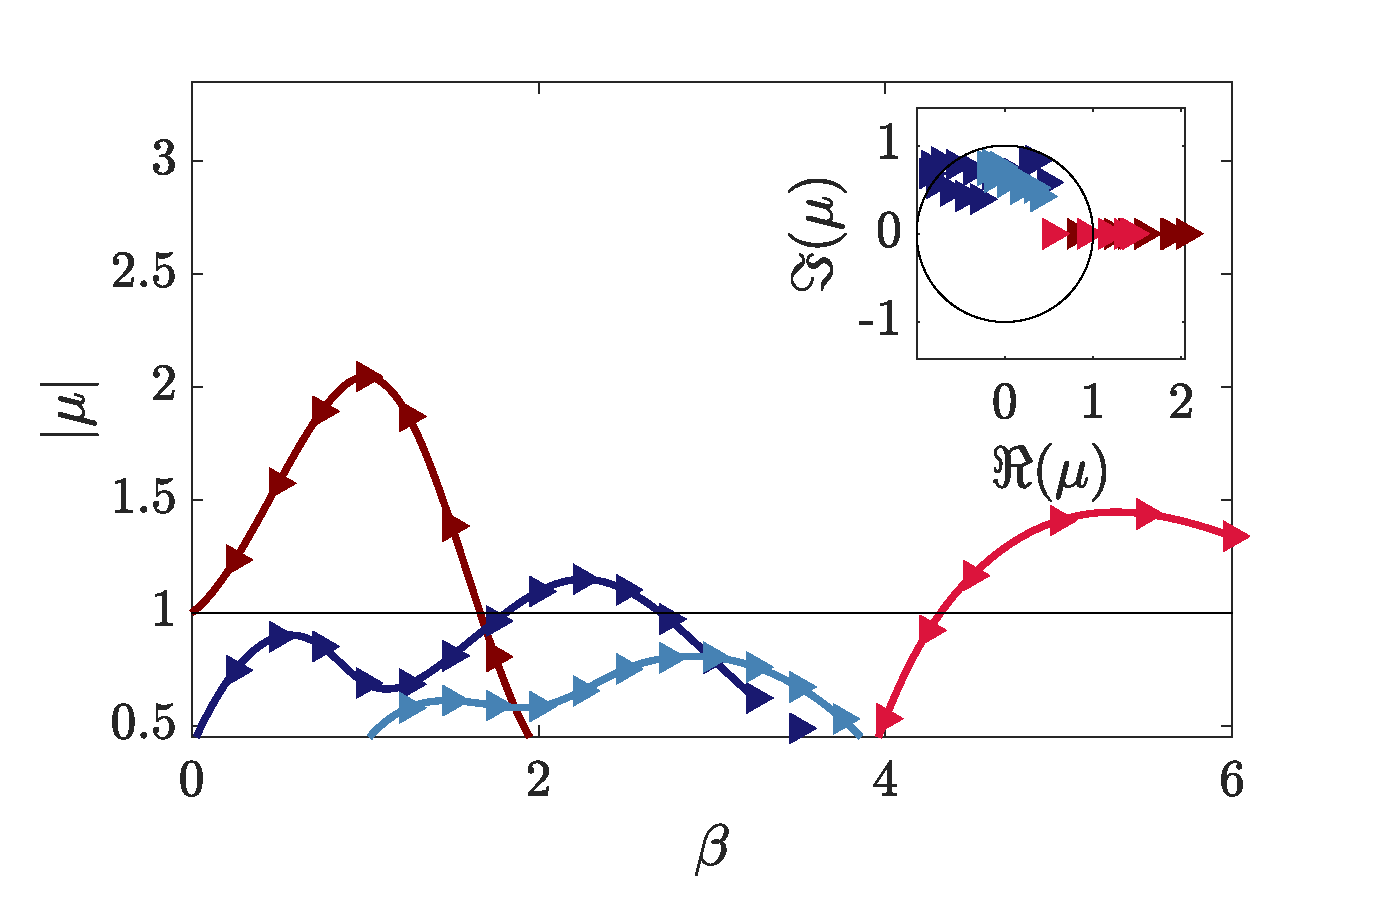
\includegraphics[width=0.49\textwidth]{./fig/AR1p25/mu_beta_Re220.eps}
  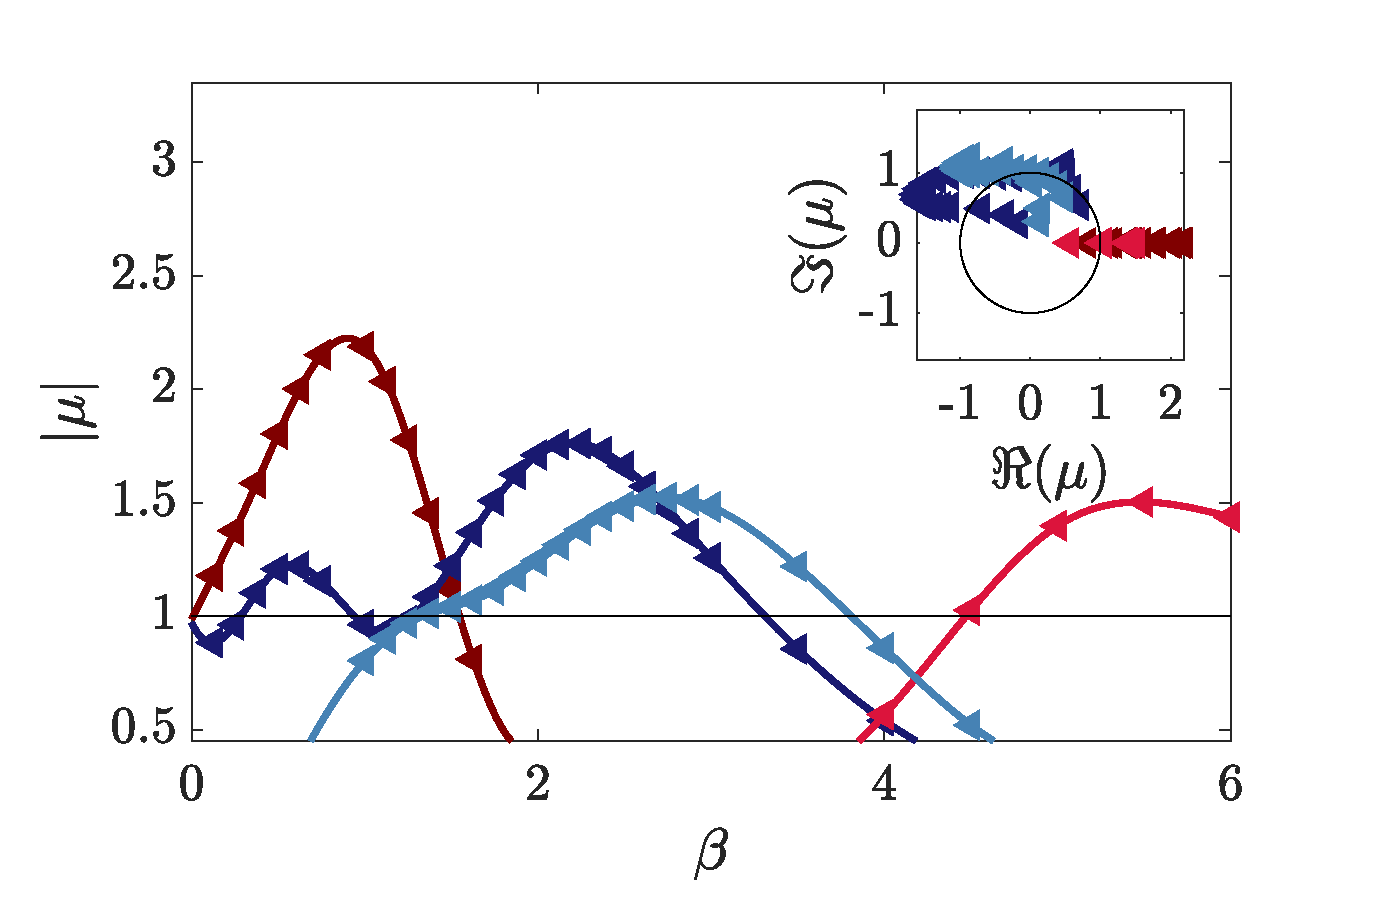
\includegraphics[width=0.49\textwidth]{./fig/AR1p25/mu_beta_Re230.eps}
  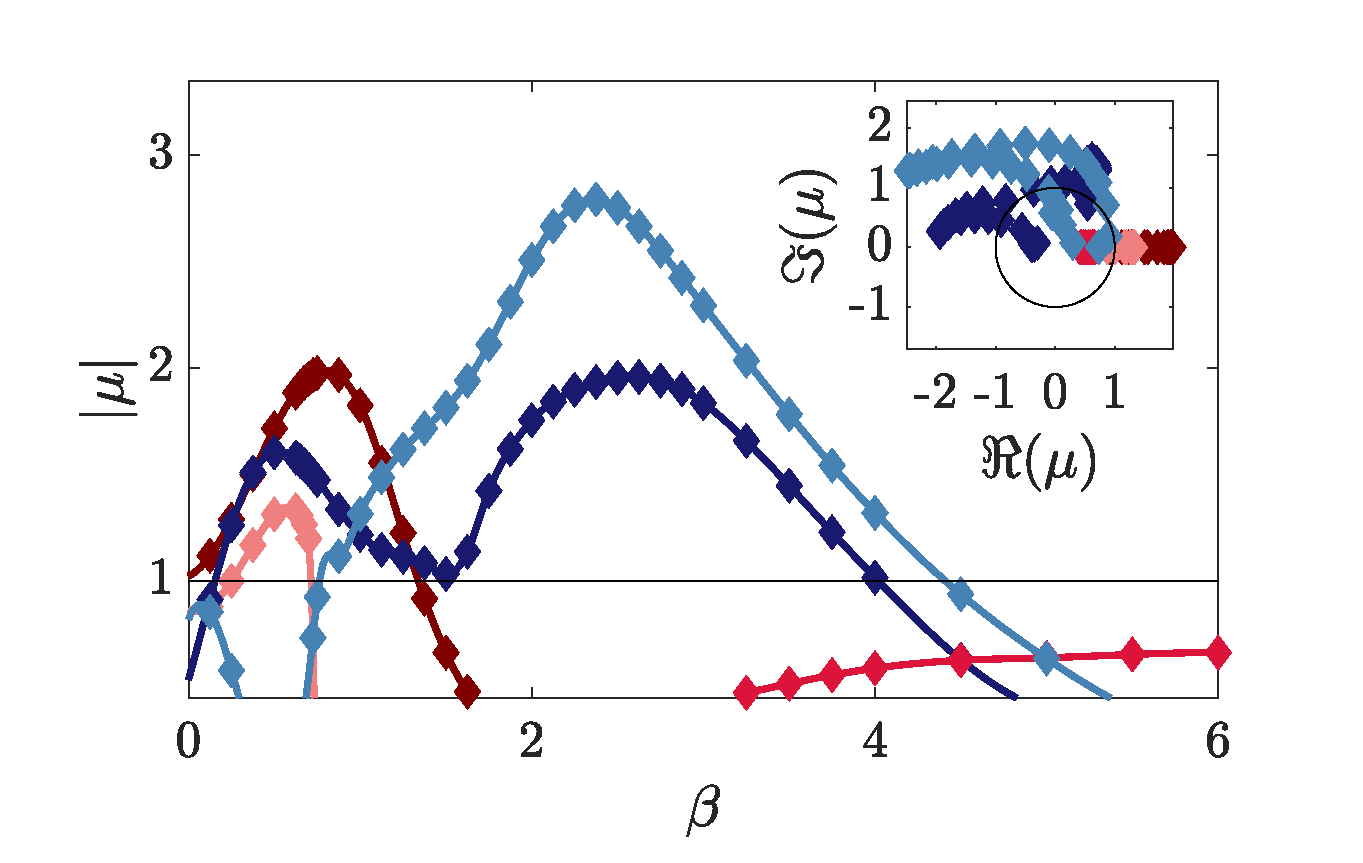
\includegraphics[width=0.49\textwidth]{./fig/AR1p25/mu_beta_Re240.eps}
  %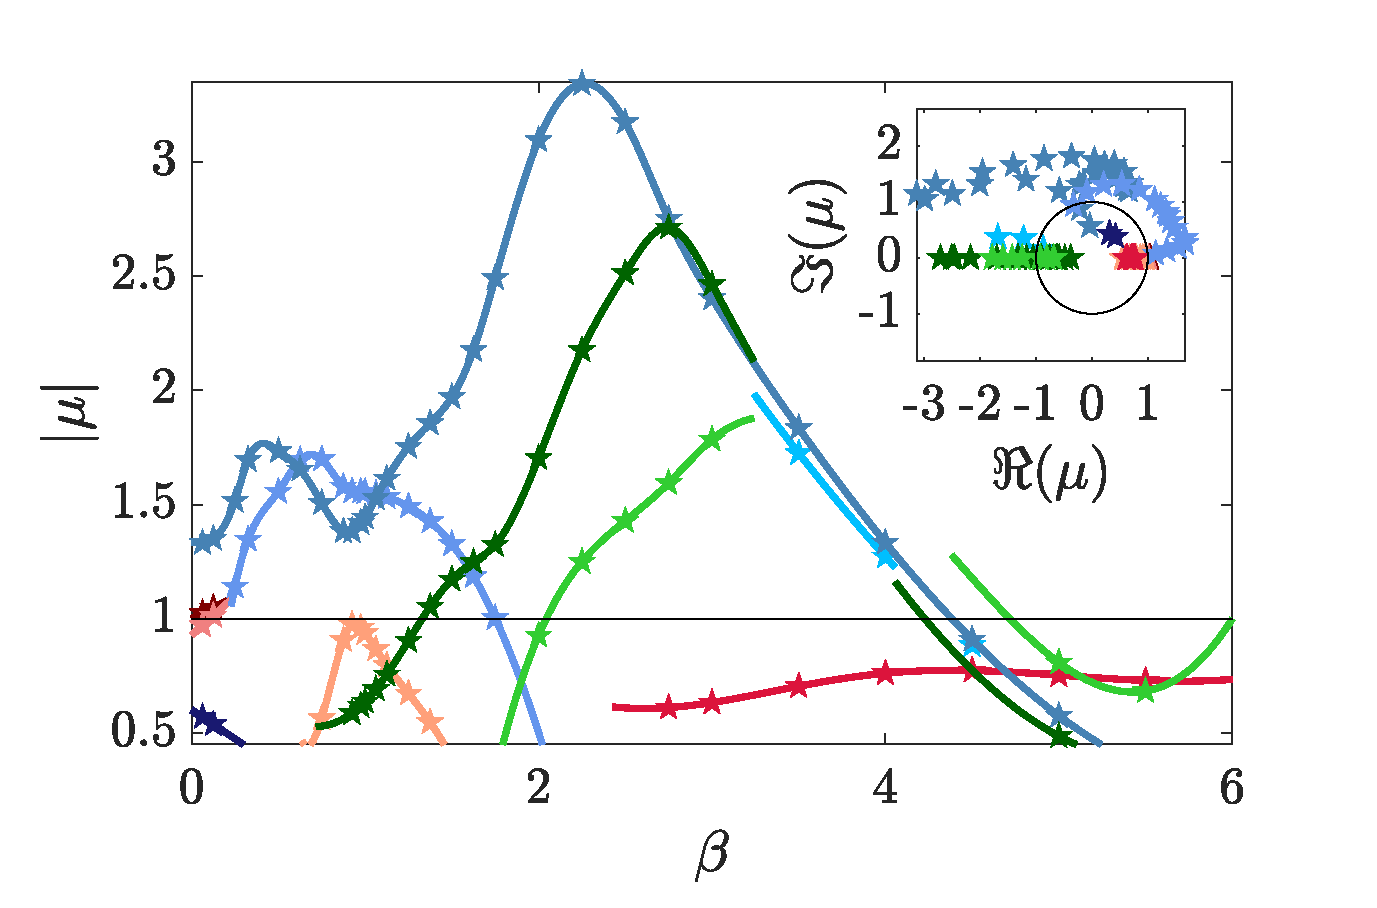
\includegraphics[width=0.49\textwidth]{./fig/AR1p25/mu_beta_Re250.eps}
  \caption{Modulus of the Floquet multipliers for $\AR=1.25$ at different $Re$. In order, the panels are for $Re=210$, $Re=220$, $Re=230$, $Re=240$ and $Re=250$. Red colour is for real and positive multipliers. Blue colour is for complex multipliers. Green colour is for real and negative multipliers. Note that for $Re=250$ at small $\beta$ we have to real, positive multipliers, associated to modes $A$ and $A'$. Then they interact and the brances collapse to a new one that has non null imaginary part. Also, in this case two new mode of subharmonic nature arise they are distinct modes, but for $\beta \approx 3$ they interact and the two branches collapse to a unique one. Then they separate again. XX ADD THE MODES XX}
\end{figure}



\begin{itemize}
  \item In this subsection we look at $\AR \in (1,2)$.
  \item Brifely recall the bifurcation scenario that has been observed for $\AR=1$, i.e. modes $A$, $QP$ and $B$.
  \item Give evidence of the influence of $\AR$ on these modes. They indeed stabilise a $\AR$ increases. Mode $B$ is not present any more for $\AR>1.25$. A new mode arises.
  \item Look at the symmetries of the modes.  
  \item \textcolor{blue}{For $\AR=1.25$ and $\AR=1.5$, modes $A$ and $B'$ become unstable is short succession. We can so use DNS to see what happens as $Re$ increases, and whether the flow changes from one mode to the other. (POD?)}
  \item Maybe we should add also $\AR=2$ and $\AR=2.5$ to see what happens.
\end{itemize}
